%%%%%%%%%%%%%%%%%%%%%%%%%%%%%%%%%%%%%%%%%%  不使用 authblk 包制作标题  %%%%%%%%%%%%%%%%%%%%%%%%%%%%%%%%%%%%%%%%%%%%%%
%-------------------------------PPT Title-------------------------------------
\title{20-多体相互作用}
%-----------------------------------------------------------------------------
%----------------------------Author & Date------------------------------------

%\author[\textrm{Jun\_Jiang}]{姜\;\;骏\inst{}} %[]{} (optional, use only with lots of authors)
%% - Give the names in the same order as the appear in the paper.
%% - Use the \inst{?} command only if the authors have different
%%   affiliation.
%\institute[BCC]{\inst{}%
\institute[Gain~Strong]{\inst{}%
%\vskip -20pt 北京市计算中心}
\vskip -20pt {\large 格致斯创~科技}}
\date[\today] % (optional, should be abbreviation of conference name)
{%	{\fontsize{6.2pt}{4.2pt}\selectfont{\textcolor{blue}{E-mail:~}\url{jiangjun@bcc.ac.cn}}}
\vskip 45 pt {\fontsize{8.2pt}{6.2pt}\selectfont{%清华大学\;\;物理系% 报告地点
	\vskip 5 pt \textrm{2023.09.16}}}
}

%% - Either use conference name or its abbreviation
%% - Not really information to the audience, more for people (including
%%   yourself) who are reading the slides onlin%%   yourself) who are reading the slides onlin%%   yourself) who are reading the slides onlineee
%%%%%%%%%%%%%%%%%%%%%%%%%%%%%%%%%%%%%%%%%%%%%%%%%%%%%%%%%%%%%%%%%%%%%%%%%%%%%%%%%%%%%%%%%%%%%%%%%%%%%%%%%%%%%%%%%%%%%

\subject{}
% This is only inserted into the PDF information catalog. Can be left
% out.
%\maketitle
\frame
{
%	\frametitle{\fontsize{9.5pt}{5.2pt}\selectfont{\textcolor{orange}{“高通量并发式材料计算算法与软件”年度检查}}}
\titlepage
}
%-----------------------------------------------------------------------------

%------------------------------------------------------------------------------列出全文 outline ---------------------------------------------------------------------------------
%\section*{}
%\frame[allowframebreaks]
%{
%  \frametitle{Outline}
%%  \frametitle{\textcolor{mycolor}{\secname}}
%  \tableofcontents%[current,currentsection,currentsubsection]
%}
%%在每个section之前列出全部Outline
%%类似的在每个subsection之前列出全部Outline是\AtBeginSubsection[]
%\AtBeginSection[]
%{
%  \frame<handout:0>%[allowframebreaks]
%  {
%    \frametitle{Outline}
%%全部Outline中,本部分加亮
%    \tableofcontents[current,currentsection]
%  }
%}

%-----------------------------------------------PPT main Body------------------------------------------------------------------------------------
\small
%\section{\rm{VASP~}软件中\rm{PAW~}计算的实现}
%\frame
%
%	\frametitle{\textrm{VASP}计算的特色}
%	相比于与普通的第一原理计算软件,\textrm{VASP}很好地平衡了计算效率和精度的问题,总的来说,\textrm{VASP}主要通过这几个特色保证了计算的高效能
%	\begin{itemize}
%	     \item 迭代与优化算法的多样性\\
%		     本质上电荷密度迭代 \textrm{\&\&} 体系总能量优化是相同的优化问题,采用了类似的算法\upcite{CMS6-15_1996,PRB54-11169_1996}:\\
%			\textcolor{blue}{\textrm{Pseudo-Newton、Conjugate-Gradient、Broyden~mix、damping-factor、RMM-DIIS}}
%	     \item 尽可能采用局域基(原子轨道基)函数:~\\
%		     \textcolor{blue}{\textrm{LREAL}}=\textcolor{red}{\textrm{.TRUE.}}\\
%			优化的投影函数也尽可能在实空间表示
%	     \item \textrm{PAW}原子数据集:\textcolor{blue}{优异的赝势}\upcite{PRB59-1758_1999}
%	\end{itemize}
%}
\section{\rm{Green's function}}
\frame
{
	\frametitle{多重散射与\textrm{Green's function}}
\begin{figure}[h!]
	\vspace{-0.55in}
\centering
%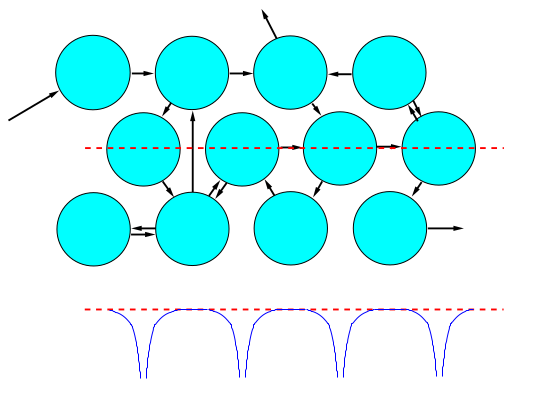
\includegraphics[height=1.80in,width=1.95in,viewport=5 0 515 495,clip]{Figures/multiple-scattering_theory.png}
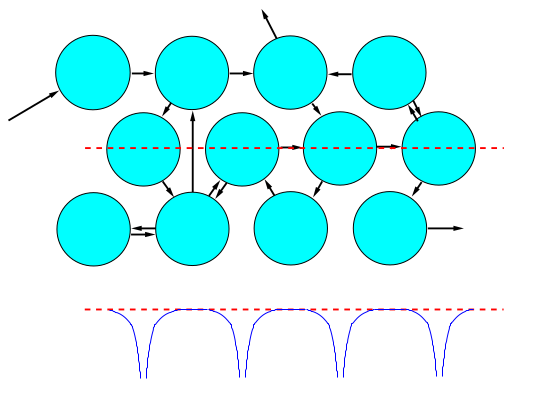
\includegraphics[height=2.32in,width=2.48in,viewport=5 0 515 475,clip]{Figures/multiple-scattering_theory.png}
\caption{\tiny \textrm{Central idea of multiple scattering theory:~ decomposition of electronic motion into scattering at atomic sites and free-electron like propagation in between. The bottom of the figure gives a sketch for the potential along the dashed line.}}
\label{Multi-scattering}
\end{figure}
\textcolor{blue}{多重散射:~}入射波是\textcolor{red}{所有来自其他散射中心的出射波叠加}
			\begin{displaymath}
				\begin{aligned}
					\tilde G=&\tilde G_0+\tilde G_0\mathbf{v}\tilde G_0+G_0\mathbf{v}\tilde G_0\mathbf{v}\tilde G_0+\cdots\\
					=&\tilde G_0+\tilde G_0\mathbf{v}\tilde G \Longrightarrow \tilde G=(\tilde G_0^{-1}-\mathbf{v})^{-1}
%					\tilde G=&(\tilde G_0^{-1}-\mathbf{t})^{-1}
				\end{aligned}
			\end{displaymath}
}

\frame
{
	\frametitle{\textrm{Green's function}}
	\begin{itemize}
\vspace{-7pt}
		\item 时间序列的\textrm{Green's function}定义为$G(\mathbf{x}_1,t_1;\mathbf{x}_2,t_2)=-\mathrm{i}\langle\Theta_N^0|\hat{\mathbf{T}}[\hat\psi(\mathbf{x}_1,t_1)\hat\psi^{\dag}(\mathbf{x}_2,t_2)]|\Theta_N^0\rangle$
		\item \textrm{Green function}的\textcolor{blue}{\textrm{Lehmann}表象}为
			\begin{displaymath}
				\begin{aligned}
					\hspace*{-35pt}
					G(\mathbf{x}_1,\mathbf{x}_2;\omega)=&\sum\limits_i\dfrac{\langle\Theta_N^0|\hat\psi_i(\mathbf{x}_1)|\Theta_{N+1}^0\rangle\langle\Theta_{N+1}^0|\hat\psi_i^{\dag}(\mathbf{x}_2)|\Theta_N^0\rangle}{\omega-(E_{N+1}^i-E_N^0)+\mathrm{i}\eta}\\
					+&\sum\limits_i\dfrac{\langle\Theta_N^0|\hat\psi_i^{\dag}(\mathbf{x}_2)|\Theta_{N-1}^0\rangle\langle\Theta_{N-1}^0|\hat\psi_i(\mathbf{x}_1)|\Theta_N^0\rangle}{\omega+(E_{N-1}^i-E_N^0)-\mathrm{i}\eta}\qquad\eta\rightarrow0^+
				\end{aligned}
			\end{displaymath}
			{\fontsize{6.2pt}{6.2pt}\selectfont{存在小的虚部$\eta$保证频率域的\textrm{Fourier}变换收敛.~这样表示的\textrm{Green's function},在复平面中的极点与增加/失去一个粒子体系的能量对应,因此也称为\textcolor{blue}{谱表象\textrm{(Spectral~representation)}}}}
	\end{itemize}
\begin{figure}[h!]
\centering
\vspace{-5pt}
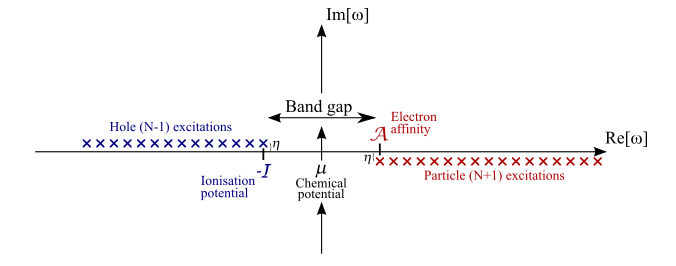
\includegraphics[height=0.80in,width=2.05in,viewport=30 1 660 265,clip]{Figures/GW-0.png}
\caption{\textrm{\tiny{The poles of the time-ordered Green's function.}}}%(与文献\cite{EPJB33-47_2003}图1对比)
\label{GW-0}
\end{figure}
}

\frame
{
	\frametitle{\textrm{Green's function}}
{\fontsize{7.8pt}{6.2pt}\selectfont{
	用\textrm{Green's function}表示的电荷密度为
	\begin{displaymath}
		\rho(\vec rt)=-\mathrm{i}\mathop{\mathrm{lim}}\limits_{\tau\rightarrow 0^{\dag}}\int G(\mathbf{x}t,\mathbf{x}t+\tau)\mathrm{d}\xi
	\end{displaymath}
	体系总能~\textrm{(Galistsii-Migdal公式)}
	\begin{displaymath}
		E=\frac12\int\mathrm{d}\mathbf{x}\mathop{\mathrm{lim}}\limits_{t^{\prime}\rightarrow t^{\dag}}\left[\frac{\partial}{\partial t}-\mathrm{i}h(\mathbf{x})\right]G(\mathbf{x},t;\mathbf{x}^{\prime},t^{\prime})_{\mathbf{x}^{\prime}\rightarrow x}
	\end{displaymath}
	将\textrm{Lehmann}表象的分母改写
	\begin{displaymath}
		\begin{aligned}
			&\omega-(E_{N+1}^i-E_N)+\mathrm{i}\eta\\
			=&\omega-(E_{N+1}^i-E_{N+1}^0)-(E_{N+1}^0-E_N^0)+\mathrm{i}\eta\\
			\approx&\omega-(E_{N+1}^i-E_{N+1}^0)-\mu+\mathrm{i}\eta\\
			&\omega+(E_{N-1}^i-E_N)-\mathrm{i}\eta\\
			=&\omega+(E_{N-1}^i-E_{N-1}^0)+(E_{N-1}^0-E_N^0)-\mathrm{i}\eta\\
			\approx&\omega+(E_{N-1}^i-E_{N-1}^0)+\mu-\mathrm{i}\eta
		\end{aligned}
	\end{displaymath}
	这里化学势$\mu$的定义为
	\begin{displaymath}
		\dfrac{E_{N+1}^0-E_N^0}{1}\approx\dfrac{\mathrm{d}E}{\mathrm{d}N}\bigg|_N=\mu(N)\approx\mu(N-1):=\mu
	\end{displaymath}
}}
}

\frame
{
	\frametitle{\textrm{Green's function}与\textrm{Spectral function}}
	谱函数\textrm{(Spectral function)}的定义为
	\begin{displaymath}
		\begin{aligned}
			A(\mathbf{x},\mathbf{x}^{\prime};\omega)=&-\dfrac1{\pi}\mathrm{Im}G(\mathbf{x},\mathbf{x}^{\prime};\omega)\\
%			=&\sum_ig_i(\mathbf{x})g_i^{\ast}(\mathbf{x}^{\prime})\delta(\omega+E_N^0-E_{N+1}^i)\\
%			&+f_i(\mathbf{x})f_i^{\ast}(\mathbf{x}^{\prime})\delta(\omega+E_{N-1}^i-E_{N}^0)\\
			=&-\frac1{\pi}\frac{\textcolor{green}{\mathrm{Im}\Sigma}}{(\omega-\varepsilon_i-\textcolor{red}{\mathrm{Re}\Sigma})^2+(\textcolor{green}{\mathrm{Im}\Sigma})^2}
		\end{aligned}
	\end{displaymath}
	物理上,谱函数$A(\mathbf{x},\mathbf{x}^{\prime},\omega)$对应局域态密度\textrm{(local density of state)}
\begin{figure}[h!]
%	\vspace{-5pt}
\centering
%\vspace{-10pt}
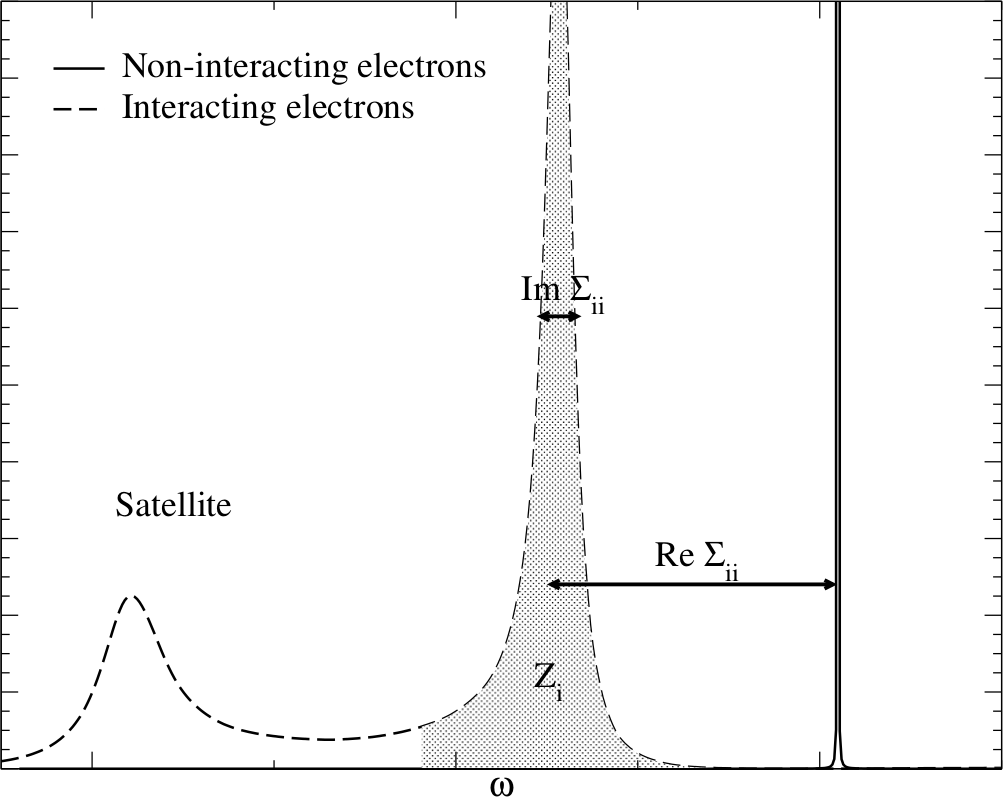
\includegraphics[height=1.4in,width=2.00in,viewport=0 0 1050 800,clip]{Figures/GW_spectral-function.png}
%\caption{\textrm{\small{The relation of the varibous Green's function.}}}%(与文献\cite{EPJB33-47_2003}图1对比)
\label{Spectral_function}
\end{figure}
}

\frame
{
	\frametitle{\textrm{Green's function}与\textrm{Hamiltonian}}
	\begin{itemize}
		\item \textrm{Green's function}是\textrm{Hamiltonian}的\textcolor{blue}{翻转}
			\begin{displaymath}
				1=(\omega-H)G\Longleftrightarrow G^{-1}=(\omega -H)
			\end{displaymath}
		\item \textrm{Lehmann}表象下,\textrm{Kohn-Sham}(无相互作用、忽略自旋的)\textrm{Hamiltonian}对应的\textrm{Green' function}
			\begin{displaymath}
				G_{\textcolor{magenta}{0}}(\vec r,\vec r^{\prime};\omega)=\sum_i\dfrac{\psi_i(\vec r)\psi_i^{\ast}(\vec r^{\prime})}{\omega-\varepsilon_i+\mathrm{i}\eta\mathrm{sgn}(\varepsilon_n-\mu)}
			\end{displaymath}
			{\fontsize{6.2pt}{6.2pt}\selectfont{
				\begin{displaymath}
					\mbox{这里}\quad\varepsilon_i=\left\{
					\begin{aligned}
						&E_{N-1}^0-E_{N-1}^i\\
						&E_{N+1}^i-E_{N+1}^0
					\end{aligned}\right.\quad\psi_i(\vec r)\left\{
						\begin{aligned}
							&\langle\Theta_{N-1}^i|\hat\psi_i(\vec r)|\Theta_{N}^0\rangle\qquad \varepsilon<\mu\\
							&\langle\Theta_N^0|\hat\psi_i(\vec r)|\Theta_{N+1}^i\rangle\qquad \varepsilon>\mu
						\end{aligned}\right.%\qquad\mu\mbox{是体系的化学势}
				\end{displaymath}
			}}
		\item 相互作用体系的\textrm{Hamiltonian}%的\textrm{Green's function}
		\fontsize{9.5pt}{4.2pt}\selectfont{	\begin{displaymath}
			\hspace*{-35pt}	\begin{aligned}
				\underbrace{\bigg(-\dfrac{\hbar^2}{2m_e}\nabla^2+V_{\mathrm{ion}}(\vec r)+V_H(r)\bigg)}_{\mathrm{\textcolor{blue}{non-int.}}}+\textcolor{magenta}{\Sigma}(\vec r,\vec r^{\prime},\omega)=H(\omega)\Longrightarrow H_0+\textcolor{magenta}{\Sigma}(\textcolor{red}{\omega})=H(\textcolor{red}{\omega})
					 %\mathrm{energy/frequency dependent Hamiltonian}
			\end{aligned}
			\end{displaymath}}
	\end{itemize}
}

\frame
{
	\frametitle{\textrm{Dyson}方程}
	\begin{itemize}
		\item 相互作用体系的\textrm{Green's function}
\begin{displaymath}
	\begin{aligned}
		(H_0-\omega)+\Sigma(\omega)&=(H-\omega)\\
		-G_0^{-1}(\omega)+\Sigma(\omega)&=-G^{-1}(\omega)\\
	\end{aligned}
\end{displaymath}
	\end{itemize}
\begin{figure}[h!]
	\vspace{-5pt}
\centering
\animategraphics[autoplay, loop, height=1.2in]{1}{Figures/Multi_scattering-}{0}{9}
\label{Multiple_scattering-0-9}
\end{figure}
	\vspace{-0.2in}
单粒子\textrm{Green's function}传播满足\textrm{Dyson's Equation}
\begin{displaymath}
	\textcolor{blue}{G^{-1}(\omega)=G_0^{-1}(\omega)-\Sigma(\omega)}
\end{displaymath}
}

\frame
{
	\frametitle{\textrm{Green's function}的物理意义}
\fontsize{7.9pt}{4.2pt}\selectfont{
	时间序列的\textrm{Green's function}~$G(\vec r,\vec r^{\prime},t-t^{\prime})$描述了粒子由$(\vec r,t)$到$\vec r^{\prime},t^{\prime}$的传播:~假设粒子在时-空点$(\vec r,t)$位置出现,则$G(\vec r,\vec r^{\prime},t-t^{\prime})$表示在时-空点$(\vec r^{\prime},t^{\prime})$找到粒子的概率\footnote{\fontsize{6.5pt}{4.2pt}\selectfont{因此单粒子\textrm{Green's funtion}被称为传播子.}}
	\begin{displaymath}
		G_{0}(\vec r,\vec r^{\prime};\omega)=\sum_n^{\mathrm{all}}\dfrac{\langle N|\psi_n^{\ast}(\vec r)\psi_n^{\dag}(\vec r^{\prime})|N\rangle}{\omega-\varepsilon_n+\mathrm{i}\eta\mathrm{sgn}(\varepsilon_n-\mu)}
	\end{displaymath}
\begin{figure}[h!]
	\vspace{-0.12in}
\centering
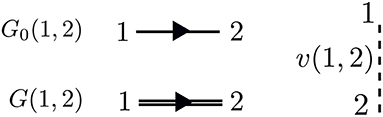
\includegraphics[height=0.50in,width=1.74in,viewport=0 0 415 125,clip]{Figures/DFT_GW-3.jpg}
%\caption{\tiny \textrm{Central idea of multiple scattering theory:~ decomposition of electronic motion into scattering at atomic sites and free-electron like propagation in between. The bottom of the figure gives a sketch for the potential along the dashed line.}}
\label{Green's_function-physical interpretation}
\end{figure}
	\begin{itemize}
		\item 粒子传播子:~$G_0(1,2)=G_0(\vec r_1,\vec r_2,t_2-t_1)$且\textcolor{blue}{$(t_2>t_1)$}
			\begin{displaymath}
				G_0(1,2)=\sum_n^{\textcolor{blue}{\mathrm{vir.}}}\psi_n^{\ast}(\vec r_1)\psi_n(\vec r_2)\mathrm{e}^{-\mathrm{i}(\varepsilon_n-\mu)(\textcolor{blue}{t_2-t_1})}
			\end{displaymath}
		\item 空穴传播子:~$G_0(1,2)$且\textcolor{blue}{$(t_1>t_2)$}
			\begin{displaymath}
				G_0(1,2)=\sum_n^{\textcolor{blue}{\mathrm{occ.}}}\psi_n^{\ast}(\vec r_1)\psi_n(\vec r_2)\mathrm{e}^{-\mathrm{i}(\varepsilon_n-\mu)(\textcolor{blue}{t_1-t_2})}
			\end{displaymath}
	\end{itemize}}
}

\frame
{
	\frametitle{传播子与自能}
\begin{figure}[h!]
	\vspace{-0.13in}
\centering
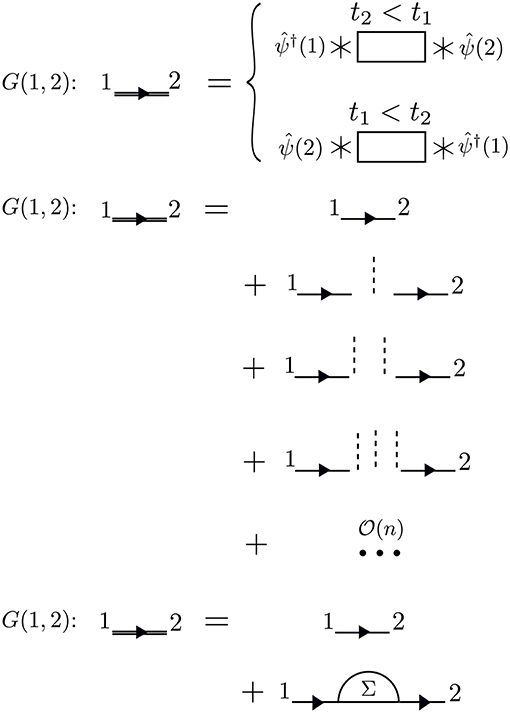
\includegraphics[height=2.88in,width=2.10in,viewport=0 0 510 715,clip]{Figures/DFT_GW-4.jpg}
%\caption{\tiny \textrm{Central idea of multiple scattering theory:~ decomposition of electronic motion into scattering at atomic sites and free-electron like propagation in between. The bottom of the figure gives a sketch for the potential along the dashed line.}}
\label{Green's_function-physical-interaction}
\end{figure}
}

\frame
{
	\frametitle{激发与光学带隙}
\begin{figure}[h!]
\centering
\vspace{-10pt}
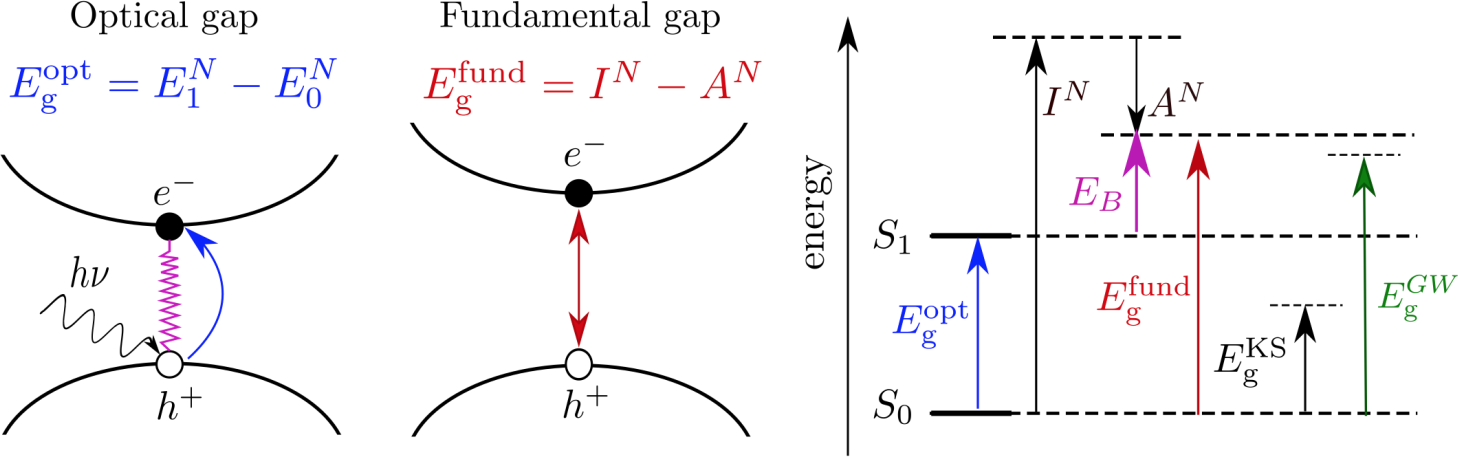
\includegraphics[height=1.3in,width=4.00in,viewport=0 0 1470 470,clip]{Figures/Green_function-Gap.png}
%\caption{\textrm{\small{The relation of the varibous Green's function.}}}%(与文献\cite{EPJB33-47_2003}图1对比)
\label{GW-Optical_Gap}
\end{figure}
\begin{displaymath}
		\underbrace{E_{\textrm{g}}^{\mathrm{KS}}}_{\textrm{\tiny KS~gap}}~=~\varepsilon_{\mathrm{LUMO}}^{\mathrm{KS}}-\varepsilon_{\mathrm{HOMO}}^{\mathrm{KS}}~\ll~\underbrace{\textcolor{green}{E_{\mathrm{g}}^{GW}}}_{\textcolor{green}{\tiny GW~\textrm{gap}}} ~=~\varepsilon_{\mathrm{LUMO}}^{GW}-\varepsilon_{\mathrm{HOMO}}^{GW}
\end{displaymath}
\begin{displaymath}
		\underbrace{\textcolor{blue}{E_{\textrm{g}}^{\mathrm{opt}}}}_{\textcolor{blue}{\textrm{\tiny optical~gap}}}~=~\varepsilon_1^{\mathrm{N}}-\varepsilon_0^{\mathrm{N}}~=~\underbrace{\textcolor{red}{E_{\mathrm{g}}^{\mathrm{fund}}}}_{\textcolor{red}{\textrm{\tiny fundamental~gap}}}+\underbrace{\textcolor{purple}{E_{\mathrm{B}}}}_{\textcolor{purple}{\textrm{\tiny excitionic effect}}}
\end{displaymath}
}

\frame
{
	\frametitle{\textrm{Green's function}与动态屏蔽}
	\vspace*{-15pt}
	\begin{itemize}
		\item 单粒子\textrm{Green's~function}:
	\begin{displaymath}
		\textcolor{blue}{G}(\vec r_1,\vec r_2;\textcolor{brown}{\omega})=\underbrace{\sum_i\dfrac{\psi_i(\vec r_1)\psi_i(\vec r_2)}{\textcolor{brown}{\omega}-\varepsilon_i-\mathrm{i}\eta}}_{\textcolor{green}{\mathrm{removal~part~=~IPs}}}+\underbrace{\sum_a\dfrac{\psi_a(\vec r_1)\psi_a(\vec r_2)}{\textcolor{brown}{\omega}-\varepsilon_a+\mathrm{i}\eta}}_{\textcolor{red}{\mathrm{addition~part~=~EAs}}}
	\end{displaymath}
\item 极化函数:
	\begin{displaymath}
		P(\vec r_1,\vec r_2;\textcolor{brown}{\omega})=-\dfrac{\mathrm{i}}{\pi}\int\textcolor{blue}{G}(\vec r_1,\vec r_2;\textcolor{brown}{\omega}+\omega^{\prime})\textcolor{blue}{G}(\vec r_1,\vec r_2;\omega^{\prime})\mathrm{d}\omega^{\prime}
	\end{displaymath}
\item 介电函数:
	\begin{displaymath}
		\epsilon(\vec r_1,\vec r_2;\textcolor{brown}{\omega})=\delta(\vec r_1-\vec r_2)-\int\dfrac{P(\vec r_1,\vec r_2;\textcolor{brown}{\omega})}{\textcolor{purple}{|\vec r_2-\vec r_3|}}\mathrm{d}\vec r_3
	\end{displaymath}
\item 动态屏蔽\textrm{Coulomb}势
	\begin{displaymath}
		\textcolor{cyan}{W}(\vec r_1,\vec r_2;\textcolor{brown}{\omega})=\int\dfrac{\epsilon^{-1}(\vec r_1,\vec r_3;\textcolor{brown}{\omega})}{\textcolor{purple}{|\vec r_2-\vec r_3|}}\mathrm{d}\vec r_3
	\end{displaymath}
	\end{itemize}
}

\frame
{
	\frametitle{微观介电函数与宏观介电函数}
	介电函数$\epsilon(\vec r_1,\vec r_2;\omega)$在倒空间表示为
	\begin{displaymath}
		\begin{aligned}
			\epsilon_{\vec G_1,\vec G_2}(\vec q,\omega)=&\delta(\vec G_1-\vec G_2)-\int\textcolor{purple}{\frac{4\pi}{|\vec G_2+\vec q||\vec G_3+\vec q|}}P_{\vec G_1,\vec G_2}(\vec q,\omega)\mathrm{d}\vec G_3\\
			=&\delta(\vec G_1-\vec G_2)-\textcolor{purple}{v(\vec G_2)}P_{\vec G_1,\vec G_2}\qquad \vec G_1,\vec G_2\neq0
		\end{aligned}
	\end{displaymath}
	\textrm{RPA}近似下,宏观介电函数$\epsilon_M(\omega)$与微观介电函数$\epsilon(\vec q,\omega)$的关系
	\begin{displaymath}
		\frac1{\epsilon_M(\omega)}\equiv\mathop{\mathrm{lim}}\limits_{\vec q\rightarrow0}\epsilon_{0,0}^{-1}(\vec q,\omega)
	\end{displaymath}
	不难看出,如果微观介电函数矩阵是非对角化的,宏观介电函数的每个矩阵元都有来自微观介电函数的矩阵元的贡献\footnote{\fontsize{7.0pt}{6.2pt}\selectfont{这称为局域场效应\textrm{(local field effects)}}}。特殊地,对于均匀电子气,微观介电函数是对角化的,可有
	\begin{displaymath}
		\epsilon_M(\omega)\approx\mathop{\mathrm{lim}}\limits_{\vec q\rightarrow0}\epsilon_{0,0}(\vec q,\omega)
	\end{displaymath}
}

\frame
{
	\frametitle{宏观介电函数与屏蔽极化函数}
	宏观介电函数$\epsilon_M(\omega)$还可以用屏蔽极化函数$\bar{P}$表示
	\begin{displaymath}
		\epsilon_M(\omega)=1-\mathop{\mathrm{lim}}\limits_{\vec q\rightarrow0}[v_0(\vec q)\bar{P}_{0,0}(\vec q,\omega)]
	\end{displaymath}
	这里屏蔽极化函数$\bar{P}$与极化函数$P$满足类似\textrm{Dyson}方程
	\begin{displaymath}
		\bar{P}=P+P\bar{v}\bar{P}
	\end{displaymath}
	并且在倒空间$\bar{v}$取为
	\begin{displaymath}
		\bar{v}_{\vec G}(\vec q)=\left\{
			\begin{aligned}
				&0 &\vec G=0\\
				v_{\vec G}(\vec q)=&\frac{4\pi}{|\vec q+\vec G|^2} \quad&\vec G\neq0
			\end{aligned}\right.
	\end{displaymath}
	在能量损失谱理论中,响应函数$\chi$也有类似\textrm{Dyson}方程的关系式\footnote{\fontsize{6.1pt}{4.2pt}\selectfont{习惯上,吸收/发射光谱中响应函数称极化函数,符号用$P(\omega)$;~电子能量损失谱中响应函数称固有极化函数,符号用$\chi(\omega)$.两者都可以用宏观介电函数表示,没有本质区别.}}
\begin{displaymath}
	\chi=P+Pv\chi
\end{displaymath}
}

\frame
{
	\frametitle{原子基表示的动态屏蔽}
	\begin{itemize}
		\item 电子排斥积分\textrm{(Electron repulsion integrals~(ERIs))}
			\begin{displaymath}
				(pq|rs)=\iint\dfrac{\psi_p(\vec r_1)\psi_q(\vec r_1)\psi_r(\vec r_2)\psi_s(\vec r_2)}{|\vec r_1-\vec r_2|}\mathrm{d}\vec r_1\vec r_2
			\end{displaymath}
		\item $\textcolor{cyan}{W}$的谱表象
{\fontsize{7.0pt}{6.2pt}\selectfont{			\begin{displaymath}
				\begin{aligned}
					\hspace*{-35pt}
					\textcolor{cyan}{W}_{pq,rs}(\textcolor{brown}{\omega})=&\iint\psi_p(\vec r_1)\psi_q(\vec r_1)\textcolor{cyan}{W}(\vec r_1,\vec r_2;\textcolor{brown}{\omega})\psi_r(\vec r_2)\psi_s(\vec r_2)\mathrm{d}\vec r_1\mathrm{d}\vec r_2\\
					=&\underbrace{(pq|rs)}_{\textrm{(static)~exchange~part}}+\underbrace{2\sum_m\textcolor{violet}{(pq|m)(rs|m)}\bigg[\dfrac1{\textcolor{brown}{\omega}-\textcolor{orange}{\Omega_m^{\textrm{RPA}}}+\mathrm{i}\eta}-\dfrac1{\textcolor{brown}{\omega}+\textcolor{orange}{\Omega_m^{\textrm{RPA}}}-\mathrm{i}\eta}\bigg]}_{\mathrm{(dynamical)~correlation~part~~\textcolor{cyan}{W}_{pq,rs}^c(\textcolor{brown}{\omega})}}
				\end{aligned}
			\end{displaymath}}}
		\item 屏蔽电子排斥积分(谱权重)
			\begin{displaymath}
				\textcolor{violet}{(pq|m)}=\sum_{ia}(pq|ia)(\textcolor{orange}{\mathbf{X}_m^{\mathrm{RPA}}}+\textcolor{orange}{\mathbf{Y}_m^{\mathrm{RPA}}})_{ia}
			\end{displaymath}
	\end{itemize}
}

\frame
{
	\frametitle{动态屏蔽的计算}
	\begin{itemize}
		\item 直接\textrm{RPA}计算\textrm{(pseudo-hermitian linear problem)}
			\begin{displaymath}
				\begin{aligned}
					\begin{pmatrix}
						\mathbf{A}^{\mathrm{RPA}} &\mathbf{B}^{\mathrm{RPA}}\\
						-\mathbf{B}^{\mathrm{RPA}} &-\mathbf{A}^{\mathrm{RPA}}\\
					\end{pmatrix}
					\cdot
					\begin{pmatrix}
						\textcolor{orange}{	\mathbf{X}_m^{\mathrm{RPA}}}\\
						\textcolor{orange}{\mathbf{Y}_m^{\mathrm{RPA}}}
					\end{pmatrix}=\Omega_{m}^{\mathrm{RPA}}
					\begin{pmatrix}
						\textcolor{orange}{	\mathbf{X}_m^{\mathrm{RPA}}}\\
						\textcolor{orange}{\mathbf{Y}_m^{\mathrm{RPA}}}
					\end{pmatrix}
				\end{aligned}
			\end{displaymath}
			{\fontsize{9.0pt}{6.2pt}\selectfont{对于单粒子态,有
				\begin{displaymath}
					\mathbf{A}_{ia,ib}^{\mathrm{RPA}}=\delta_{ij}\delta_{ab}(\varepsilon_a-\varepsilon_i)+2(ia|bj)\qquad \mathbf{B}_{ia,ib}^{\mathrm{RPA}}=2(ia|jb)
				\end{displaymath}}}
		\item \textrm{Non-hermitian to hermitian}
			\begin{displaymath}
				(\mathbf{A}-\mathbf{B})^{1/2}\cdot(\mathbf{A}+\mathbf{B})\cdot(\mathbf{A}-\mathbf{B})^{1/2}\cdot\mathbf{Z}_m=\Omega_m^2\mathbf{Z}_m
			\end{displaymath}
			\begin{displaymath}
				\begin{aligned}
					(\mathbf{X}_m+\mathbf{Y}_m)=\Omega_m^{-1/2}(\mathbf{A}-\mathbf{B})^{+1/2}\cdot\mathbf{Z}_m\\
					(\mathbf{X}_m-\mathbf{Y}_m)=\Omega_m^{+1/2}(\mathbf{A}-\mathbf{B})^{-1/2}\cdot\mathbf{Z}_m\\
				\end{aligned}
			\end{displaymath}
		\item \textrm{Tamm-Damcoff}近似\textrm{(TDA)}
			\begin{displaymath}
				\mathbf{B}=\mathbf{0}\Longrightarrow \mathbf{A}\cdot\textcolor{orange}{\mathbf{X}_m}=\textcolor{orange}{\Omega_m^{\mathrm{TDA}}\mathbf{X}_m}
			\end{displaymath}
	\end{itemize}
}

\section{\rm{GW}近似}
\frame
{
	\frametitle{准粒子:~激发与屏蔽}
\begin{figure}[h!]
	\vspace{-0.12in}
\centering
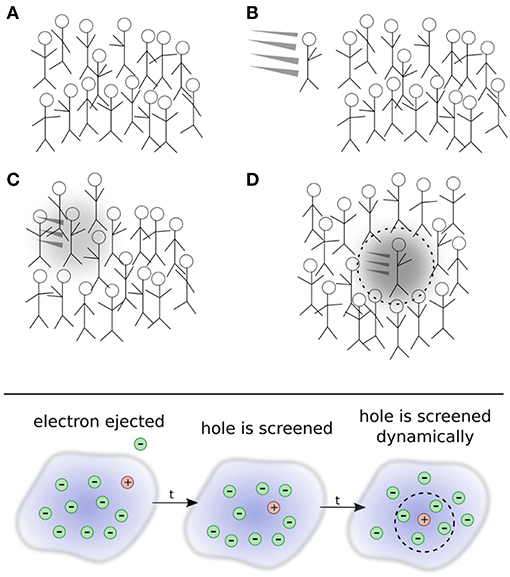
\includegraphics[height=2.65in,width=2.25in,viewport=0 0 510 575,clip]{Figures/DFT_GW-2.jpg}
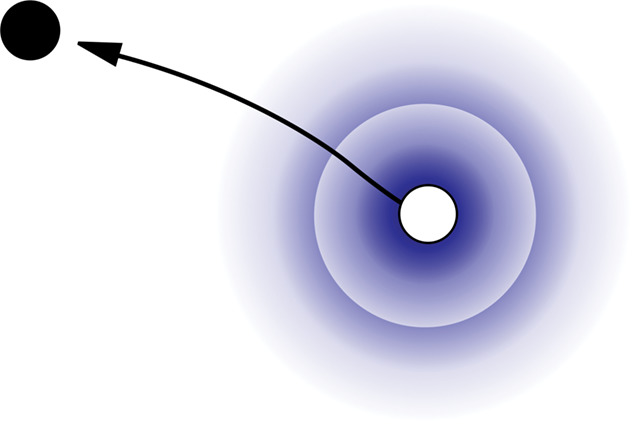
\includegraphics[height=1.80in,width=1.65in,viewport=0 0 455 525,clip]{Figures/DFT_GW-electron.jpg}
\label{Green's_function-quasi-particle}
\end{figure}
}

\frame
{
	\frametitle{准粒子与自能的计算}
	即使是单粒子\textrm{Green's function}也无法精确求解,必须作适当近似:\\
	{\fontsize{7.0pt}{6.2pt}\selectfont{一个合理的近似是写成\textrm{Kohn-Sham}本征态和本征值表示的\textrm{Lehmann}形式$G_{\mathrm{KS}}^0(\vec r_1,\vec r_2;\textcolor{brown}{\omega})$}}\\
	再由\textrm{Dyson}方程得到相互作用的\textrm{Green's function}
	\begin{displaymath}
		\hspace*{-13pt}
		[\textcolor{blue}{G}(\vec r_1,\vec r_2;\textcolor{brown}{\omega})]^{-1}=\underbrace{[G_{\mathrm{KS}}^0(\vec r_1;\vec r_2;\textcolor{brown}{\omega})]^{-1}}_{\mathrm{KS~Green's~function}}+\textcolor{red}{\Sigma^{\mathrm{XC}}}(\vec r_1,\vec r_2;\textcolor{brown}{\omega})-\underbrace{v^{\mathrm{XC}}(\vec r_1)}_{\mathrm{KS~potential}}\delta(\vec r_1-\vec r_2)
	\end{displaymath}
	{\fontsize{7.2pt}{6.2pt}\selectfont{\textrm{Dyson}方程描述了相互作用体系$G$通过自能$\Sigma$与独立体系$G_0$(传播子)关联}}
	\begin{itemize}
		\item 自能$\Sigma$含时、非局域(非\textrm{Hermitian}),故准粒子能量为复数
			\begin{displaymath}
				\textcolor{brown}{\omega}=\varepsilon_p^{\mathrm{KS}}+\textcolor{red}{\Sigma_{pp}^{\mathrm{XC}}}(\textcolor{brown}{\omega})-V_p^{\mathrm{XC}}\qquad{\tiny \mbox{记~~$V_p^{\mathrm{XC}}=\int\psi_p(\vec r)v^{\mathrm{XC}}\psi_p(\vec r)\mathrm{d}\vec r$}}
			\end{displaymath}
%	\textrm{Dyson}方程
%	\begin{displaymath}
%		\begin{aligned}
%	&G(\vec r_1,t_1;\vec r_2,t_2)=G_0(\vec r_1,t_1;\vec r_2,t_2)\\
%	&+\int G_0(\vec r_1,t_1;\vec r_3,t_3)\Sigma(\vec r_3,t_3;\vec r_4,t_4)G(\vec r_4,t_4;\vec r_2,t_2)\mathrm{d}t_3\mathrm{d}\vec r_3\mathrm{d}t_4\mathrm{d}\vec r_4
%		\end{aligned}
%	\end{displaymath}

		\item 求解含有自能$\Sigma$的准粒子\textrm{(quasi-particle, QP)}方程,可以求解得到多体体系中重整化电子的量子态(\textrm{Hedin}方程)
%			$$\bigg[\hat h_0(\vec r_1)+v_H(\vec r_1)\bigg]\Psi(\vec r_1)+\int\textcolor{red}{\Sigma(\vec r_1,\vec r_2;\omega^{\mathrm{QP}})}\Psi(\vec r_2)\mathrm{d}\vec r_2=\varepsilon^{\mathrm{QP}}\Psi(\vec r_1)$$
	\end{itemize}
}

\frame
{
	\frametitle{\textrm{Hedin}方程} 
	\textrm{Hedin}方程是一系列耦合的积分-微分方程组%,只能通过迭代方式来求解
	\begin{displaymath}
		\begin{aligned}
			\Sigma(\mathbf{12})=&\mathrm{i}\int G(\mathbf{13})\Gamma(\mathbf{234})W(\mathbf{41})\mathrm{d}(\mathbf{34})\\
			W(\mathbf{12})=&v(\mathbf{12})+\int v(\mathbf{13})P(\mathbf{34})W(\mathbf{42})\mathrm{d}(\mathbf{34})\\
			P(\mathbf{12})=&-\mathrm{i}\int G(\textcolor{blue}{\mathbf{13}})G(\textcolor{blue}{\mathbf{41}})\Gamma(\mathbf{342})\mathrm{d}(\textcolor{blue}{\mathbf{34}})\\
			\Gamma(\mathbf{123})=&\delta(\mathbf{12})\delta(\mathbf{13})+\int \frac{\delta\Sigma(\textcolor{red}{\mathbf{12}})}{\delta G(\textcolor{magenta}{\mathbf{45}})}G(\textcolor{magenta}{\mathbf{46}})G(\textcolor{magenta}{\mathbf{75}})\Gamma(\mathbf{673})\mathrm{d}(\textcolor{magenta}{\mathbf{4567}})
		\end{aligned}
	\end{displaymath}
	{\fontsize{7.2pt}{6.2pt}\selectfont{这里$\mathbf{1}=(\vec r_1,t_1,\xi_1)$, $v$表示净的\textrm{Coulomb}相互作用}}
{\fontsize{9.0pt}{6.2pt}\selectfont{
	\begin{itemize}
		\item 极化函数$P$:~包含体系对引入电子或空穴的响应\\
			$P$通过包括一对粒子-空穴对(两个\textrm{Green's function})来表示
		\item 顶角函数$\Gamma$:~包含空穴-电子的 相互作用\\
			反过来,$\Gamma$是由空穴-电子相互作用的激发引起的势函数的变化来确定的
	\end{itemize}}}
}

\frame
{
	\frametitle{\textrm{Hedin}方程} 
	耦合的\textrm{Hedin}方程的自洽图示
\begin{figure}[h!]
\centering
\vspace{-10pt}
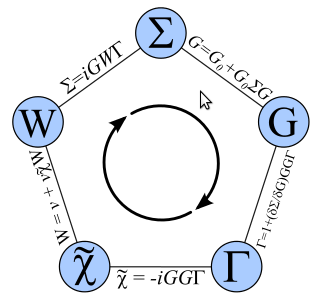
\includegraphics[height=2.2in,width=2.25in,viewport=5 5 330 335,clip]{Figures/GW-1.png}
%\caption{\textrm{\small{The relation of the varibous Green's function.}}}%(与文献\cite{EPJB33-47_2003}图1对比)
\label{GW-1}
\end{figure}
	直接求解\textrm{Hedin}方程是非常复杂的,有必要采取近似(把$\Gamma$函数表达成可分离的$\delta$函数),这就是$GW$近似
}

%\frame
%{
%	\frametitle{}
%	\begin{itemize}
%			\vspace{-15pt}
%		\item 定义不可约极化率$\tilde\chi$,$\tilde\chi(\vec r_1,t_1;\vec r_2,t_2)\equiv\dfrac{\delta n(\vec r_1,t_1)}{\delta U_{e\!f\!f}(\vec r_2,t_2)}=-\mathrm{i}\dfrac{\delta G(\vec r_1,t_1,\vec r_1,t_1+\eta)_{\eta\rightarrow0}}{\delta U_{e\!f\!f}(\vec r_2,t_2)}$
%		\item 定义动态屏蔽相互作用$W(\vec r_1,t_1;\vec r_2,t_2)\equiv\int\epsilon^{-1}(\vec r_1,t_1;\vec r_3,t_3)v(\vec r_3,r_3;\vec r_2,t_2)\mathrm{d}t_3\mathrm{d}\vec r_3$
%		\item 介电矩阵与不可约极化率满足关系:
%			\begin{displaymath}
%				\begin{aligned}
%					&\epsilon(\vec r_1,t_1;\vec r_2,t_2)\\
%					=&\delta(\vec r_1,t_1;\vec r_2,t_2)-\int v(\vec r_,t_1,\vec r_3,t_3)\tilde\chi(\vec r_3,t_3;\vec r_2,t_2)\mathrm{d}t_3\mathrm{d}\vec r_3
%				\end{aligned}
%			\end{displaymath}
%	\end{itemize}
%}

\frame
{
	\frametitle{$GW$近似:~\textrm{Vertex function}函数的简化}
\vspace{-20pt}
	$$\Gamma(\vec r_{12},t_{12};\vec r_3t_3)\approx\delta(\vec r_1,t_1;\vec r_2,t_2)\delta(\vec r_1,t_1;\vec r_3,t_3)\equiv\Gamma^{GW}(\vec r_{12},t_{12};\vec r_3,r_3)$$
\begin{figure}[h!]
\vspace{-8pt}
\centering
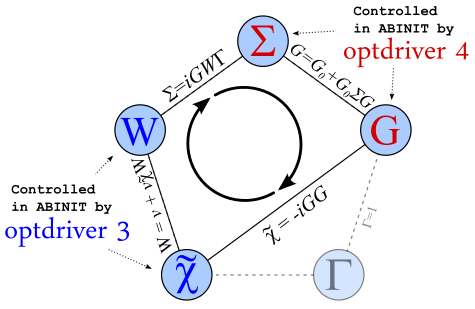
\includegraphics[height=1.50in,width=2.45in,viewport=5 5 530 320,clip]{Figures/GW-3.png}
%\caption{\textrm{\small{The relation of the varibous Green's function.}}}%(与文献\cite{EPJB33-47_2003}图1对比)
\label{GW-2}
\end{figure}
频率空间内,$GW$近似的自能表示为
%$$\Sigma(\vec r_1,\vec r_2;\omega)=\dfrac{\mathrm i}{2\pi}\int \mathrm e^{\mathrm i\omega^{\prime}\delta^+}G(\vec r_1,\vec r_2;\omega+\omega^{\prime})W(\vec r_1,\vec r_2;\omega^{\prime})\mathrm{d}\omega^{\prime}$$
{\fontsize{7.2pt}{6.2pt}\selectfont{
\begin{displaymath}
	\hspace*{-12pt}
	\underbrace{\textcolor{red}{\Sigma^{\mathrm{XC}}}(\vec r_1,\vec r_2;\textcolor{brown}{\omega})}_{GW~\mathrm{self-energy}}=\underbrace{\textcolor{purple}{\Sigma^{\mathrm{X}}}(\vec r_1,\vec r_2)}_{\mathrm{exchange}}+\underbrace{\textcolor{red}{\Sigma^{\mathrm{C}}}(\vec r_1,\vec r_2;\textcolor{brown}{\omega})}_{\mathrm{correlation}}=\dfrac{\mathrm i}{2\pi}\int\textcolor{blue}{G}(\vec r_1,\vec r_2;\textcolor{brown}{\omega}+\omega^{\prime})\textcolor{cyan}{W}(\vec r_1,\vec r_2;\omega^{\prime})\mathrm{e}^{\mathrm{i}\eta\omega^{\prime}}\mathrm{d}\omega^{\prime}
\end{displaymath}
交换部分(\textcolor{blue}{静态自能}): $\textcolor{purple}{\Sigma_{pq}^{\mathrm{X}}}=-\sum\limits_i(pi|iq)$\\
相关部分(\textcolor{blue}{动态自能}):
%\begin{displaymath}
	$\textcolor{red}{\Sigma_{pq}^{\mathrm{C}}}(\textcolor{brown}{\omega})=2\sum\limits_{im}\frac{\textcolor{violet}{(pi|m)(qi|m)}}{\textcolor{brown}{\omega}-\varepsilon_i+\textcolor{orange}{\Omega_m^{\mathrm{RPA}}}-\mathrm{i}\eta}+2\sum\limits_{am}\frac{\textcolor{violet}{(pa|m)(qa|m)}}{\textcolor{brown}{\omega}-\varepsilon_a-\textcolor{orange}{\Omega_m^{\mathrm{RPA}}}+\mathrm{i}\eta}$
%\end{displaymath}
}}
}

\frame
{
	\frametitle{由$GW$到$G_0W_0$近似}
	自洽迭代求解$GW$耦合方程组仍非常复杂,通常须作进一步近似,典型如 $G_0W_0$近似:
	\vskip 6pt
{\fontsize{9.0pt}{6.2pt}\selectfont{
	准粒子的波函数用\textrm{KS}本征态近似,并构造准粒子\textrm{Green's function}~$G_0^{\mathrm{KS}}$,屏蔽极化函数计算采用\textrm{RPA}近似:
	$$\tilde{\chi}^0(\vec r_1,t_1;\vec r_2,t_2)=-\mathrm{i}G_0^{\mathrm{KS}}(\vec r_1,t_1;\vec r_2,t_2)G_0^{\mathrm{KS}}(\vec r_1,t_1;\vec r_2,t_2)$$
在此基础上,可得到体系的自能
	$$\Sigma(\vec r_1,t_1;\vec r_2,t_2)=\mathrm{i}G_0^{\mathrm{KS}}W_0(\vec r_1,t_1+\eta;\vec r_2,t_2)_{\eta\rightarrow0}$$
\vskip 3pt
	准粒子能量$\varepsilon^{GW}$则可由$\varepsilon^{\mathrm{KS}}$通过自能线性展开近似
{\fontsize{7.6pt}{6.2pt}\selectfont{
	\begin{displaymath}
		\hspace*{-14pt}
		\textcolor{red}{\Sigma_{pp}^{\mathrm{XC}}}(\textcolor{brown}{\omega})\approx\textcolor{red}{\Sigma_{pp}^{\mathrm{XC}}}(\varepsilon_p^{\mathrm{KS}})+(\textcolor{brown}{\omega}-\varepsilon_p^{\mathrm{KS}})\frac{\partial\textcolor{red}{\Sigma_{pp}^{\mathrm{XC}}}(\textcolor{brown}{\omega})}{\partial\textcolor{brown}{\omega}}\bigg|_{\textcolor{brown}{\omega}=\varepsilon_p^{\mathrm{KS}}}\Longrightarrow	\textcolor{blue}{\varepsilon_p^{GW}}=\varepsilon_p^{\mathrm{KS}}+\textcolor{green}{Z_p}[\textcolor{red}{\Sigma_{pp}^{\mathrm{XC}}}(\varepsilon_p^{\mathrm{KS}})-v_p^{\mathrm{XC}}]
	\end{displaymath}}}
	这里$\textcolor{green}{Z_p}$称为重整化因子
	\begin{displaymath}
		\underbrace{\textcolor{green}{Z_p}}_{\mathrm{renormalization~factor}}\equiv\bigg[1-\frac{\partial\textcolor{red}{\Sigma_{pp}^{\mathrm{XC}}}(\textcolor{brown}{\omega})}{\partial\textcolor{brown}{\omega}}\bigg|_{\textcolor{brown}{\omega}=\varepsilon_p^{\mathrm{KS}}}\bigg]^{-1}\qquad{\tiny \mbox{要求~~$0\leqslant\textcolor{green}{Z_p}\leqslant1$}}
	\end{displaymath}}}
}

\frame
{
	\frametitle{$G_0W_0$计算流程}
\begin{figure}[h!]
	\vspace{-0.17in}
\centering
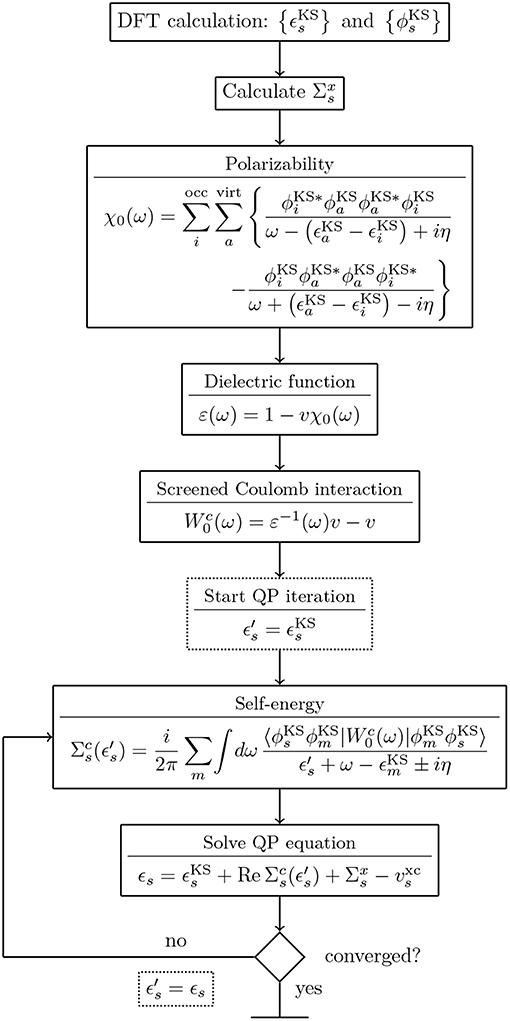
\includegraphics[height=2.78in,width=1.50in,viewport=0 0 510 1035,clip]{Figures/Flowchart-for-a-G0W0-calculation-starting-from-a KS-DFT-calculation.jpg}
\caption{\tiny \textrm{A flowchart for a $G_0W_0$ calculation starting from a KS-DFT calculation.}}
\label{G0W0_flowchart}
\end{figure}
}

\frame
{
	\frametitle{$GWA$与\textrm{LDA+}$U$}
	\begin{displaymath}
		\begin{aligned}
			V_{m\sigma}^{GWA}=&\sum_{m^{\prime}\sigma^{\prime}}U_{mm^{\prime}}^0n_{m^{\prime}\sigma^{\prime}}-U_{mm}^0n_{m\sigma}-\sum_{m^{\prime}\neq m}J_{mm^{\prime}}n_{m^{\prime}\sigma}\\
			+&\left( \frac12-n_{m\sigma} \right)\sum_{m^{\prime}}W_{mm^{\prime}}
		\end{aligned}
	\end{displaymath}
	其中$U_{mm^{\prime}}^0$是\textcolor{blue}{未屏蔽\textrm{Coulomb~}相互作用矩阵},$J_{mm^{\prime}}$是\textcolor{blue}{交换矩阵}\\
	$W_{mm^{\prime}}$是\textcolor{red}{电子相关作用的矩阵$W_{\mathrm c}(\vec r,\vec r^{\prime};0)$的矩阵元}

	定义屏蔽相互作用参数$W$
	\begin{displaymath}
		W=-\sum_{m^{\prime}}W_{mm^{\prime}}
	\end{displaymath}
	因此,$\mathrm{GWA}$近似的矩阵元表示为
	\begin{displaymath}
			V_{m\sigma}^{GWA}=\sum_{m^{\prime}\sigma^{\prime}}U_{mm^{\prime}}^0n_{m^{\prime}\sigma^{\prime}}-(U_{mm}^0-W)n_{m\sigma}-\sum_{m^{\prime}\neq m}J_{mm^{\prime}}n_{m^{\prime}\sigma}-\frac12W
	\end{displaymath}
}

\frame
{
	\frametitle{$GWA$与\textrm{LDA+}$U$}
	对应于\textrm{LSDA},势能的修正
	\begin{displaymath}
		\begin{aligned}
			\delta V_{m\sigma}=&V_{m\sigma}^{GWA}-V_{m\sigma}^{\mathrm{LSDA}}\\
			=&\sum_{m^{\prime}\sigma^{\prime}}U_{mm^{\prime}}^0n_{m^{\prime}\sigma^{\prime}}-(U_{mm^{\prime}}^0-W)n_{m\sigma}-\sum_{m^{\prime}\neq m}J_{mm^{\prime}}n_{m^{\prime}\sigma}-\frac12W\\
			-&F^0\sum_{m^{\prime}\sigma^{\prime}}n_{m^{\prime}\sigma^{\prime}}+J\sum_mn_{m\sigma}+\frac12(F^0-J)\\
			=&\sum_{m^{\prime}\sigma^{\prime}}(U_{mm^{\prime}}^0-F^0)n_{m^{\prime}\sigma^{\prime}}-(U_{mm^{\prime}}^0-W)n_{m\sigma}-\sum_{m^{\prime}\neq m}J_{mm^{\prime}}n_{m^{\prime}\sigma}\\
			-&\frac12W+J\sum_mn_{m\sigma}+\frac12(F^0-J)
		\end{aligned}
	\end{displaymath}
}

\frame
{
	\frametitle{$GWA$与\textrm{LDA+}$U$}
	\textcolor{red}{注意:~}$U_{mm^{\prime}}^0-F^0$只与\textrm{Slater~}函数$F^k(k\neq0)$有关,与$F^0$无关,并且
	\begin{displaymath}
		U_{mm^{\prime}}^0-F^0=U_{mm^{\prime}}-U
	\end{displaymath}
	这里$U=F^0-W$是屏蔽\textrm{Coulomb~}参数,$U_{mm^{\prime}}$是屏蔽\textrm{Coulomb~}矩阵
	\begin{displaymath}
		\begin{aligned}
			\delta V_{m\sigma}=&V_{m\sigma}^{GWA}-V_{m\sigma}^{\mathrm{LSDA}}\\
			=&\sum_{m^{\prime}\sigma^{\prime}}U_{mm^{\prime}}n_{m^{\prime}-\sigma}+\sum_{m^{\prime}\neq m}(U_{mm^{\prime}}-J_{mm^{\prime}})n_{m^{\prime}\sigma}\\
			-&U(N-\frac12)+J(N_{\sigma}+\frac12)
		\end{aligned}
	\end{displaymath}

	\textcolor{red}{两种方法的区别:~}\textcolor{blue}{屏蔽\textrm{Coulomb~}参数$U$的计算}
	\begin{itemize}
		\item \textrm{LDA+}$U$:~直接估计\textrm{LSDA}晶胞间相互作用
		\item $\mathrm{GWA}$:~通过复杂的响应函数计算
	\end{itemize}
}

\section{\rm{Bethe-Salpeter}方程}
\frame
{
	\frametitle{\textrm{Bethe-Salpeter}方程}
	\textrm{Bethe-Salpeter Equation~(BSE)}定量描述物质中电子-空穴对(双粒子激发)的激子效应,用于物质光吸收谱等性质的精确计算
\begin{figure}[h!]
\centering
\vspace{-5pt}
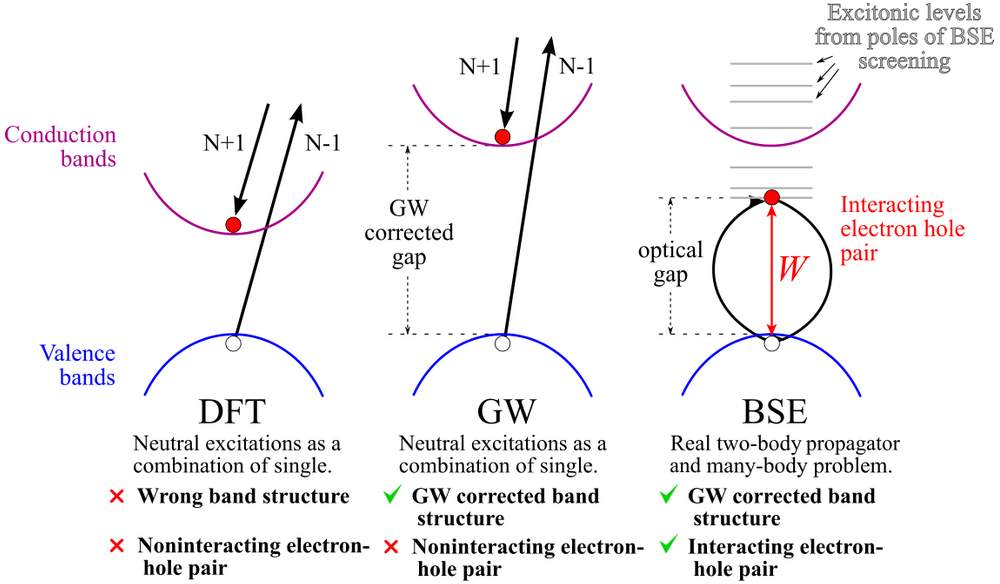
\includegraphics[height=2.45in,width=3.90in,viewport=0 0 1000 600,clip]{Figures/BSE_GW_DFT.png}
%\caption{\textrm{\tiny Feynman diagram representing the Bethe-Salpeter equation for $\chi$.}}%(与文献\cite{EPJB33-47_2003}图1对比)
\label{GW-BSE_GW_DFT}
\end{figure}
}

\frame
{
	\frametitle{\textrm{Bethe-Salpeter}方程的推导:~顶角函数的修正}
	简言之,$GW$近似是单粒子激发,极化函数$P=-\mathrm{i}GG$(\textrm{RPA}近似或$\Gamma=\delta$);~双粒子激发意味着要考虑电子-空穴吸引的影响:\\
	在$GW$基础上,利用$\Sigma=\mathrm{i}GW$,有
	\begin{displaymath}
		\Gamma(\mathbf{123})=\delta(\mathbf{12})\delta(\mathbf{13})+\mathrm{i}W(\mathbf{1}^+\mathbf{2})\int \mathrm{d}(\mathbf{67})G(\mathbf{16})G(\mathbf{72})\Gamma(\mathbf{673})
	\end{displaymath}
	{\fontsize{8.0pt}{6.2pt}\selectfont{对比\textrm{Hedin}方程,这里引入了近似$\delta\Sigma/\delta G=\mathrm{i}W$,表明:
	\begin{itemize}
		\item 激发引起屏蔽相互作用的改变$\mathrm{i}G(\delta W/\delta G)$非常小,可以忽略
		\item 实际迭代计算$\Gamma$时,可只到考虑两次迭代即可:
	\begin{displaymath}
		\Gamma^{(2)}(\mathbf{123})=\delta(\mathbf{12})\delta(\mathbf{13})+\int\mathrm{d}(\mathbf{4567})\underbrace{\textcolor{cyan}{\frac{\delta\Gamma^{(1)}(\mathbf{12})}{\delta G^{(0)}(\mathbf{45})}}}_{\textcolor{cyan}{\mathrm{i}W^{(1)}}}G^{(1)}(\mathbf{46})G^{(1)}(\mathbf{75})\Gamma^{(2)}(\mathbf{673})
	\end{displaymath}
	\end{itemize} }}
	通过$\Gamma$可有广义极化函数$\sideset{^3}{}{\mathop{P}}$
	\begin{displaymath}
		\sideset{^3}{}{\mathop{P}}(\mathbf{312})\equiv-\mathrm{i}\int\mathrm{d}(\mathbf{67})G(\mathbf{16})G(\mathbf{72})\Gamma(\mathbf{673})
	\end{displaymath}
}

\frame
{
	\frametitle{\textrm{Bethe-Salpeter}方程的推导:~四中心积分}
	对极化函数$\sideset{^3}{}{\mathop{P}}$左乘$-\mathrm{i}G(\mathbf{41})G(\mathbf{25})$并对$\mathrm{d}(\mathbf{12})$积分有
	\begin{displaymath}
		\sideset{^3}{}{\mathop{P}}(\mathbf{345})=-\mathrm{i}G(\mathbf{43})G(\mathbf{35})+\mathrm{i}\int\mathrm{d}(\mathbf{12})\textcolor{red}{G(\mathbf{41})G(\mathbf{25})W(\mathbf{1}^{+}\mathbf{2})}\sideset{^3}{}{\mathop{P}}(\mathbf{312})
	\end{displaymath}
	被积函数$GGW$是四中心形式,故极化函数可写成四中心积分$\sideset{^4}{}{\mathop{P}}$:\\
	{\fontsize{8.0pt}{6.2pt}\selectfont{
		引入屏蔽相互作用的四中心形式
		\begin{displaymath}
			\sideset{^4}{}{\mathop{W}}(\mathbf{1234})\equiv W(\mathbf{12})\delta(\mathbf{13})\delta(\mathbf{24})
		\end{displaymath}
		于是极化函数写成四中心形式
		\begin{displaymath}
			\sideset{^4}{}{\mathop{P}}=\sideset{^4}{_{\mathrm{IQP}}}{\mathop{P}}\sideset{^4}{}{\mathop{W}}\sideset{^4}{_{\mathrm{IQP}}}{\mathop{P}}
		\end{displaymath}
		四中心的准粒子极化函数$\sideset{^4}{_{\mathrm{IQP}}}{\mathop{P}}$的定义为
		\begin{displaymath}
			\sideset{^4}{_{\mathrm{IQP}}}{\mathop{P}}(\vec r_1,\vec r_2,\vec r_3,\vec r_4;\omega)=\sum_{ij}(f_i-f_j)\frac{\psi_i(\vec r_1)\psi_j^{\ast}(\vec r_2)\psi_j(\vec r_4)\psi_i^{\ast}(\vec r_3)}{\omega-\omega_{ij}+\mathrm{i}\eta}
		\end{displaymath}
		这里$\omega_{ij}=(\varepsilon_j-\varepsilon_i)$,$f_{i}$是\textrm{Fermi}占据数 }}
}

\frame
{
	\frametitle{\textrm{Bethe-Salpeter}方程的推导:~极化函数}
	于是屏蔽极化函数的四中心表示为
	\begin{displaymath}
		\begin{aligned}
			\sideset{^4}{}{\mathop{\bar{P}}}(\mathbf{1234})=&\sideset{^4}{}{\mathop{P}}(\mathbf{1234})\\
			&+\int\mathrm{d}(\mathbf{5678})\sideset{^4}{}{\mathop{P}}(\mathbf{1256})\delta(\mathbf{56})\delta(\mathbf{78})\bar{v}(\mathbf{57})
			&\times\sideset{^4}{}{\mathop{\bar{P}}}(\mathbf{7834})
		\end{aligned}
	\end{displaymath}
	由此可有$\sideset{^4}{}{\mathop{\bar{P}}}$的\textrm{Bethe-Salpeter}方程
	\begin{displaymath}
		\textcolor{blue}{\sideset{^4}{}{\mathop{\bar{P}}}=\sideset{^4}{_{\mathrm{IQP}}}{\mathop{P}}+\sideset{^4}{_{\mathrm{IQP}}}{\mathop{P}}K\sideset{^4}{}{\mathop{\bar{P}}}}
	\end{displaymath}
	这里被积函数$K$包括(1)电子-空穴交换势$\bar{v}$和(2)电子空穴吸引势$-W$
	\begin{displaymath}
		K(\mathbf{1234})=\delta(\mathbf{12})\delta(\mathbf{34})\bar{v}(\mathbf{13})-\delta(\mathbf{13})\delta(\mathbf{24})W(\mathbf{12})
	\end{displaymath}
}

\frame
{
	\frametitle{\textrm{Bethe-Salpeter}方程的推导:~极化函数}
	与屏蔽极化函数$\sideset{^4}{}{\mathop{\bar{P}}}$类似,极化函数$\sideset{^4}{}{\mathop{\chi}}$类似,只须将函数$v$替换$\bar{v}$即可.$\sideset{^4}{}{\mathop{\chi}}$的\textrm{Bethe-Salpter}方程的\textrm{Feynman}图表示如下
\begin{figure}[h!]
\centering
%\vspace{-16pt}
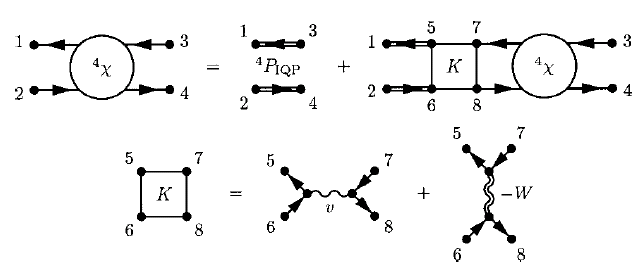
\includegraphics[height=1.5in,width=4.00in,viewport=13 15 633 260,clip]{Figures/BSE_Feynman.png}
\caption{\textrm{\tiny Feynman diagram representing the Bethe-Salpeter equation for $\chi$.}}%(与文献\cite{EPJB33-47_2003}图1对比)
\label{chi-BSE_solution}
\end{figure}
}

\frame[allowframebreaks]
{
	\frametitle{四中心的类\textrm{Dyson}方程求解$^{\ast}$}
{\fontsize{7.0pt}{6.2pt}\selectfont{
	求解四中心的类\textrm{Dyson}方程可转换成等效本征值问题,假设
	\begin{itemize}
		\item 电子-空穴对可以用等效准粒子\textrm{Hamiltonian}的本征态波函数$\psi_n$描述
		\item 电子-空穴跃迁能对应准粒子的本征值$\varepsilon_n$
		\item 初始电荷密度可由少量激发的电子-空穴对生成
		\item 这些激发准粒子的本征波函数$\psi_n$构成正交-完备基
	\end{itemize}
	于是,任意四中心函数可记作
	\begin{displaymath}
		S(\vec r_1,\vec r_1^{\prime};\vec r_1,\vec r_1^{\prime})=\sum_{n_1,\cdots,n_4}\psi_{n_1}^{\ast}(\vec r_1)\psi_{n_1}^{\ast}(\vec r_1)\psi_{n_1}^{\ast}(\vec r_1)\psi_{n_1}^{\ast}(\vec r_1)S_{(n_1n_2)(n_3n_4)}
	\end{displaymath}
	在该基组下,四中心准粒子极化函数
	\begin{displaymath}
		\sideset{^4}{_{\mathrm{IQP}}}{\mathop{P}}(\vec r_1,\vec r_2,\vec r_3,\vec r_4)=\sum_{n,n^{\prime}}(f_n-f_{n^{\prime}})\frac{\psi_n^{\ast}(\vec r_1)\psi_{n^{\prime}}(\vec r_2)\psi_{n^{\prime}}(\vec r_4)\psi_{n^{\prime}}^{\ast}(\vec r_3)}{\varepsilon_n-\varepsilon_{n^{\prime}}-\omega}
	\end{displaymath}
	是对角化的,可记为
	\begin{displaymath}
		\sideset{^4}{_{\mathrm{IQP}}}{\mathop{P}}_{(n_1n_2)(n_3n_4)}=(f_{n_2}-f_{n_1})\delta_{n_1,n_3}\delta_{n_2,n_4}/(\varepsilon_{n_2}-\varepsilon_{n_1}-\omega)
	\end{displaymath}
	如果定义函数
	\begin{displaymath}
		\bar{\Pi}\equiv[1-\sideset{^4}{_{\mathrm{IQP}}}{\mathop{P}}K]^{-1}
	\end{displaymath}
	则类\textrm{Dyson}方程变成$S=\bar{\Pi}\sideset{^4}{_{\mathrm{IQP}}}{\mathop{P}}$,而$\bar{\Pi}$在准粒子空间可表示为
	\begin{displaymath}
		\begin{aligned}
			\bar{\Pi}_{(n_1n_2)(n_3n_4)}=&[(\varepsilon_{m_2}-\varepsilon_{m_1}-\omega)\delta_{m_1,m_3}\delta_{m_2,m_4}\\
			&+(f_{m_1}-f_{m_2})K_{(m_1m_2)(m_3m_4)}]^{-1}_{(n_1n_2)(n_3n_4)}\\
			&\times(\varepsilon_{n_4}-\varepsilon_{n_3}-\omega)
		\end{aligned}
	\end{displaymath}
	定义有效双粒子\textrm{Hamiltonian}
	\begin{displaymath}
		H_{(n_1n_2)(n_3n_4)}^{2p}\equiv(\varepsilon_{n_2}-\varepsilon_{n_1})\delta_{n_1,n_3}\delta_{n_2,n_4}+(f_{n_1}-f_{n_2})K_{(n_1n_2)(n_3n_4)}
	\end{displaymath}
	于是四中心函数可以表示为
	\begin{displaymath}
		S_{(n_1n_2)(n_3n_4)}=[H^{2p}-I\omega]_{(n_1n_2)(n_3n_4)}^{-1}(f_{n_4}-f_{n_3})
	\end{displaymath} 
	而准粒子空间展开的有效\textrm{Hamiltonian}的形式为
	\begin{displaymath}
		H_{(n_1n_2)(n_3n_4)}^{2p}=
		\begin{pmatrix}
			\textcolor{red}{\mathbf{A}} &\mathbf{B}\\
			0 &\mathbf{D}
		\end{pmatrix}
	\end{displaymath}
	$\mathbf{A}$、$\mathbf{B}$、$\mathbf{D}$的具体表达形式,参阅文献\cite{RMP74-601_2002}
\vskip 3pt
具体求解$H_{(n_1n_2)(n_3n_4)}^{2p}$的本征态方程时,将仅考虑电子-空穴对贡献有关部分\footnote{\fontsize{6.5pt}{4.2pt}\selectfont{这部分称为共振部分\textrm{(resonsant part)}},描述的是与吸收频率$\omega$对应的价带-导带激发.}记作
\begin{displaymath}
	H_{(vc)(v^{\prime}c^{\prime})}^{2p,\mathrm{res}}\equiv(\varepsilon_c-\varepsilon_v)\delta_{vv^{\prime}}\delta_{cc^{\prime}}+K_{(vc)(v^{\prime}c^{\prime})}
\end{displaymath}
共振部分仅存在于$\textcolor{red}{\mathbf{A}}$中:
\begin{displaymath}
	\textcolor{red}{\mathbf{A}}=
\begin{pmatrix}
	H_{(vc)(v^{\prime}c^{\prime})}^{2p,\mathrm{res}} &K_{(vc)(v^{\prime}c^{\prime})}\\
	-[K_{(vc)(v^{\prime}c^{\prime})}]^{\ast} &-[H_{(vc)(v^{\prime}c^{\prime})}^{2p,\mathrm{res}}]^{\ast}\\
\end{pmatrix}
\end{displaymath}
取$(n_3n_4)=\{c^{\prime}v^{\prime}\}\mbox{\textrm{and}}\{v^{\prime}c^{\prime}\}$,此时任意四中心函数$S_{(n_1n_2)(n_3n_4)}$可以写成形如
\begin{displaymath}
	\textcolor{blue}{M_{(n_1n_2)(n_3n_4)}^{-1}}=[\textcolor{blue}{H^{2p}}-I\omega]_{(n_1n_2)(n_3n_4)}^{-1}
\end{displaymath}
如果记$\textcolor{cyan}{A_{\omega}}=\textcolor{cyan}{A}-I\omega$,则对照上述对四中心函数$S$的讨论,后面关注的将是$\textcolor{cyan}{A_{\omega}^{-1}}$,换言之,后面只讨论有物理意义的电子-空穴(初始\textrm{Bloch}态占据数分别为1和0)对,因此这里将用有效双粒子\textrm{Hamiltonian}$H^{2p}$指代$\mathbf{A}$部分
\vskip 3pt
一般说,$\mathbf{A}$部分具有非\textrm{Hermiitian}性,主要分成四块(两部分):
\begin{itemize}
	\item 矩阵对角块的两部分:~由电子-空穴跃迁能$\varepsilon_n$和相互作用项$K$构成
	\item 矩阵非对角块两部分:~仅有相互作用$K$构成
\end{itemize}
\begin{displaymath}
	H^{2p}=\begin{pmatrix}
		H^{2p,\mathrm{res}} &\textcolor{blue}{H^{\mathrm{coupling}}}\\	
		\textcolor{blue}{-[H^{\mathrm{coupling}}]^{\ast}} &\textcolor{magenta}{-[H^{2p,\mathrm{res}}]^{\ast}}
	\end{pmatrix}
\end{displaymath}
{\fontsize{5.0pt}{4.2pt}\selectfont{其中共振部分有\textrm{Hermiitian}性:$(H^{2p,\mathrm{res}})^{\ast}=(H^{2p,\mathrm{res}})^{T}$,耦合部分有对称性:$H^{\mathrm{coupling}}=(H^{\mathrm{coupling}})^{T}$,而$\textcolor{magenta}{-[H^{2p,\mathrm{res}}]^{\ast}}$称为反共振部分。如忽略共振部分,称为\textrm{Tamm-Dancoff}近似}}
\vskip 3pt
如果双粒子有效\textrm{Hamiltonian}~$H^{2p}$的本征态$A_{\lambda}$和本征值$E_{\lambda}$满足
\begin{displaymath}
	H^{2p}A_{\lambda}=E_{\lambda}A_{\lambda}
\end{displaymath}
则该\textcolor{magenta}{双粒子有效\textrm{Hamiltonian}之逆}的谱表示为
\begin{displaymath}
	[H^{2p}-I\omega]_{(n_1n_2)(n_3n_4)}^{-1}=\sum_{\lambda,\lambda^{\prime}}\dfrac{A_{\lambda}^{n_1n_2}N_{\lambda,\lambda}^{-1}A_{\lambda}^{\ast(n_3n_4)}}{E_{\lambda}-\omega}
\end{displaymath}
这里$N_{\lambda,\lambda^{\prime}}$是重叠矩阵(源于$H^{2p}$的非正交本征态$A_{\lambda}^{(n_1n_2)}$):
\begin{displaymath}
	N_{\lambda,\lambda^{\prime}}\equiv\sum_{n_1,n_2}A_{\lambda}^{\ast(n_1n_2)}A_{\lambda}^{(n_1n_2)}
\end{displaymath} }}
最后可以宏观介电函数的表达式为
\begin{displaymath}
	\begin{aligned}
		\epsilon_M(\omega)=&1-\mathop{\mathrm{lim}}\limits_{\vec q\rightarrow0}v(\vec q)\sum_{\lambda,\lambda^{\prime}}\left(\sum_{n_1,n_2}\langle n_1|\mathrm{e}^{-\mathrm{i}\vec q\cdot\vec r}|n_2\rangle\right.\\
		&\times\dfrac{A_{\lambda}^{(n_1n_2)}}{\omega-E_{\lambda}+\mathrm{i}\eta}N_{\lambda,\lambda^{\prime}}^{-1}\\
		&\left.\times\sum_{n_3,n_4}\langle n_4|\mathrm{e}^{\mathrm{i}\vec q\cdot\vec r^{\prime}}|n_3\rangle A_{\lambda^{\prime}}^{\ast(n_3n_4)}(f_{n_3}-f_{n_4})\right)
	\end{aligned}
\end{displaymath}
}

\frame
{
	\frametitle{\textrm{Bethe-Salpeter}方程的求解}
	具体求解$\sideset{^4}{}{\mathop{\bar{P}}}$的\textrm{Bethe-Salpter}方程时,如果$W$取为静态屏蔽\textrm{Coulomb}相互作用,则相应地$K$对应于含时屏蔽的\textrm{Hartree-Fock}近似。参照四中心的类\textrm{Dyson}方程求解过程,定义\textrm{Bethe-Salpeter}方程的有效双粒子\textrm{Hamiltonian},可有本征态方程
	\begin{displaymath}
		\begin{aligned}
			\sum_{n_3n_4}&\{(\varepsilon_{n_2}-\varepsilon_{n_1})\delta_{n_1n_3}\delta_{n_2n_4}+(f_{n_1}-f_{n_2})[\bar{v}_{(n_1n_2)(n_3n_4)}\\
			&-W_{(n_1n_2)(n_3n_4)}]\}A_{\lambda}^{(n_3n_4)}=E_{\lambda}A_{\lambda}^{(n_1n_2)}
		\end{aligned}
	\end{displaymath}
	四中心积分$\bar{v}$和$W$用四个准粒子波函数轨道$n_1,\cdots,n_4$表示:
	\begin{displaymath}
		\begin{aligned}
			\bar{v}_{(n_1n_2)(n_3n_4)}=&\langle n_1n_2|\bar{v}|n_3n_4\rangle\\	
			W_{(n_1n_2)(n_3n_4)}=&\langle n_1n_2|\bar{v}|n_3n_4\rangle	
		\end{aligned}
	\end{displaymath}
{\fontsize{8.5pt}{6.2pt}\selectfont{
类似地,有效双粒子\textrm{Hamiltonian}~$H^{2p}$的共振部分有\textrm{Hermitian}属性,且本征态波函数$A_{\lambda}$正交,则宏观介电函数为:
	\begin{displaymath}
		\textcolor{red}{\epsilon_M(\omega)=1-\mathop{\mathrm{lim}}\limits_{\vec q\rightarrow0}v_0(\vec q)\sum_{\lambda}\dfrac{\big|\sum\limits_{n_1,n_2}\langle n_1|\mathrm{e}^{-\mathrm{i}\vec q\cdot\vec r}|n_2\rangle A_{\lambda}^{(n_1n_2)}\big|^2}{\omega-E_{\lambda}+\mathrm{i}\eta}}
	\end{displaymath}}}
}

\frame
{
	\frametitle{\textrm{Bethe-Salpeter}方程的求解流程}
\begin{figure}[h!]
\centering
\vspace{-10pt}
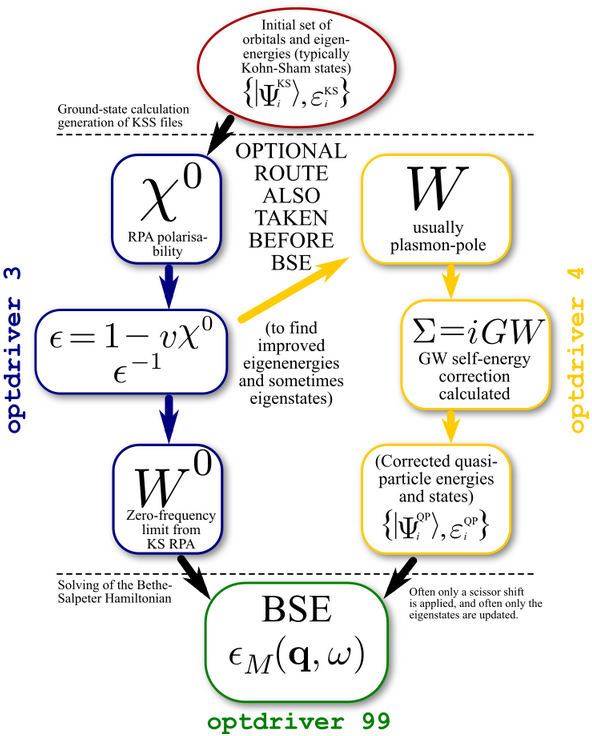
\includegraphics[height=2.75in,width=2.35in,viewport=0 0 600 735,clip]{Figures/BSE_solution.png}
\caption{\textrm{\tiny Flow diagram sketching the solution of the Bethe-Salpeter equation in practice.}}%(与文献\cite{EPJB33-47_2003}图1对比)
\label{GW-BSE_solution}
\end{figure}
}

\frame
{
	\frametitle{\textrm{DFT-GW-BSE}的本征方程}
\begin{figure}[h!]
\centering
\vspace{-10pt}
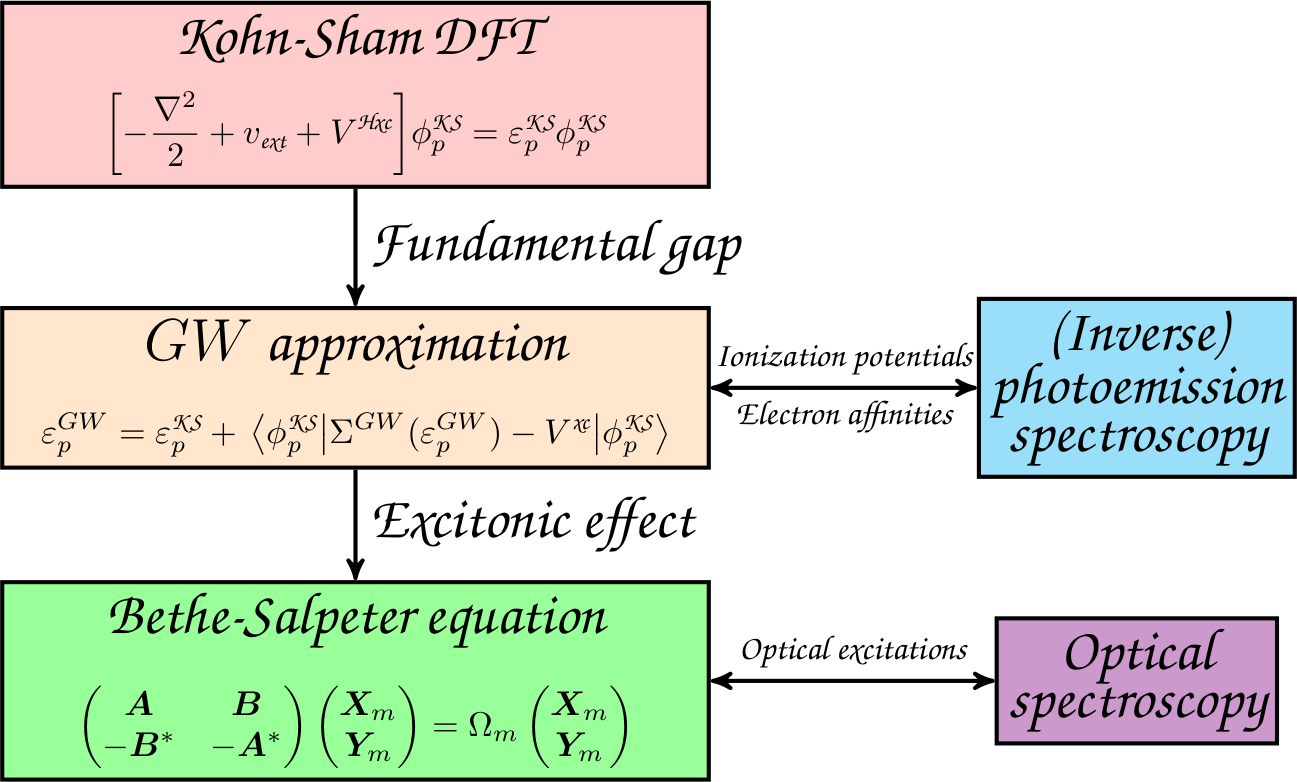
\includegraphics[height=2.65in,width=4.00in,viewport=0 0 1300 800,clip]{Figures/DFT_GW_BSE-equation.png}
%\caption{\textrm{\tiny Flow diagram sketching the solution of the Bethe-Salpeter equation in practice.}}%(与文献\cite{EPJB33-47_2003}图1对比)
\label{DFTGW-BSE_equation}
\end{figure}
}

\section{\rm{TD-DFT}}
\frame{
	\frametitle{\textrm{TD-DFT}}
	\begin{itemize}
		\item 经典的\textrm{DFT}是基态理论,不能处理激发态
	\end{itemize}
	{\fontsize{7.5pt}{4.2pt}\selectfont{如果体系所受外势随时间演化,则体系也将随之演化
			\begin{displaymath}
				A=\int_{t_0}^{t_1}\mathrm{d}t\langle\Psi(t)|\mathrm{i}\frac{\partial}{\partial t}-\hat{H}(t)|\Psi(t)\rangle
			\end{displaymath}
		根据能量最低原理,最终达到基态(体系总能极小态) ,体系演化过程中的径迹将由最小作用量$\int_{t_0}^{t_1}\mathrm{d}t\mathbf{L}(t)$决定,$\mathbf{L}$是\textrm{Lagrangian}}}\\
	与基态\textrm{DFT}的推导类似,理论上可以证明
	\begin{itemize}
		\item \textrm{Runge-Gross}定理:\\
		含时的势能与含时的密度在演化过程中有一一对应关系
	\item \textrm{von Leeuwen}定理:\\
		体系的性质有体系的密度确定,密度可通过含时\textrm{Kohn-Sham}方程得到
	\end{itemize}
	这就是含时密度泛函理论\textrm{(TD-DFT)}\\
	{\fontsize{7.5pt}{4.2pt}\selectfont{与\textrm{DFT}的交换-相关泛函类似,引入含时的交换-相关泛函,包含多体相互作用,并允许随时间演化}}
}

\frame{
	\frametitle{含时\textrm{Kohn-Sham}方程}
	{\fontsize{7.2pt}{4.2pt}\selectfont{
		\begin{itemize}
			\item 体系所受作用是密度的泛函$A[\rho]$,因此与$A[\rho]$的极值对应的\textrm{Euler}方程
	\begin{displaymath}
		\dfrac{\delta A[\rho]}{\delta\rho(\vec r,t)}=0
	\end{displaymath}
	决定了基态的含时密度(与\textrm{Hohenberg-Kohn}定理类似)
\item 引入密度为$\rho(\vec r,t)$的无相互作用体系,如体系的势函数$v$可由含时密度表示,则\\
	含时\textrm{Kohn-Sham}方程表示为
	\begin{displaymath}
		\begin{aligned}
			&\left[-\dfrac12\nabla^2+V_{\mathrm{eff}}(\vec r,t)\right]\psi_i(\vec r.t)=\mathrm{i}\dfrac{\partial}{\partial t}\psi_i(\vec r,t)\\
			&\rho(\vec r,t)=\sum_{i=1}^N|\psi_i(\vec r,t)|^2
		\end{aligned}
	\end{displaymath}
		\end{itemize}
		其中$V_{\mathrm{eff}}(\vec r,t)=V_{\mathrm{H}}(\vec r,t)+V_{\mathrm{XC}}(\vec r,t)+V_{\mathrm{ext}}(\vec r,t)$,是电子感受到的势,包括:
		\begin{itemize}
			\item 随时间演化的外势$V_{\mathrm{ext}}(\vec r,t)$
			\item 随时间演化的\textrm{Hartree}势$V_{\mathrm{H}}(\vec r,t)$
			\item 交换相关势(定义为\textcolor{blue}{体系所受作用函数与无相互作用密度的变分}):
				\begin{displaymath}
					V_{\mathrm{XC}}(\vec r,t)=\frac{\delta A_{\mathrm{XC}}[\rho]}{\delta\rho(\vec r,t)}
				\end{displaymath}
				这里$A_{\mathrm{XC}}[\rho]$是体系所受作用函数的对交换-相关有贡献的部分
		\end{itemize} }}
}

\frame
{
	\frametitle{\textrm{TD-DFT}的分类}
	\textcolor{magenta}{\textrm{TD-DFT}广泛用于电子-核体系运动的量子耦合、电磁场的量子本质,以及超导等前沿领域的研究中}
	\vskip 5pt
\textrm{TD-DFT}分为两类
\begin{itemize}
	\item \textcolor{blue}{\textrm{rt~(Real~Time)-TDDFT}}:\\
		可用于演化体系,实现动力学模拟\\
{\fontsize{7.2pt}{4.2pt}\selectfont{
用定态\textrm{Kohn-Sham}轨道$\{\phi_p^{\mathrm{opt}}(\vec r;\mathbf{R}(t))\}$展开\textrm{TD-KS}轨道,有
\begin{displaymath}
	\phi_i(\vec r,t)=\sum_{j}^{\infty}c_{ip}(t)\phi_p^{\mathrm{opt}}(\vec r;\mathbf{R}(t))
\end{displaymath}}}
	\item \textcolor{blue}{\textrm{LR~(Linear~Response)-TDDFT}}:\\
		根据体系的电子结构得到体系的光谱信息:\\
		{\fontsize{7.2pt}{4.2pt}\selectfont{不产生体系的动力学演化信息}}
	\begin{itemize}
{\fontsize{7.2pt}{4.2pt}\selectfont{
		\item 作为微扰方法,主要研究体系对含时的外部微扰的响应
		\item 含时响应与单粒子\textrm{Green's function}处理思想类似}}
	\end{itemize}
	\textrm{TD-DFT}的自洽迭代过程,可用于多体问题有关的(束缚或非束缚)激发态能量、跃迁几率等的计算
\end{itemize}
}

\frame
{
	\frametitle{响应函数}
	{\fontsize{7.8pt}{4.2pt}\selectfont{
		相互作用体系的固有极化函数(线性响应函数)$\chi$定义为
\begin{displaymath}
	\chi(\vec r,t;\vec r^{\prime},t^{\prime})=\frac{\delta\rho(\vec r,t)}{\delta V_{\mathrm{ext}}(\vec r^{\prime},t^{\prime})}\bigg|_{v_{\mathrm{ext}}=0}
\end{displaymath}
类似地,假想\textrm{Kohn-Sham}体系(无相互作用体系)的线性响应函数$\chi_0$定义为
\begin{displaymath}
	\chi_0(\vec r,t;\vec r^{\prime},t^{\prime})=\frac{\delta\rho(\vec r,t)}{\delta V_{\mathrm{eff}}(\vec r^{\prime},t^{\prime})}\bigg|_{v_{\mathrm{eff}}=0}
\end{displaymath}
利用链式关系$\delta\rho/\delta V_{\mathrm{ext}}=(\delta\rho/\delta V_{\mathrm{eff}})\times(\delta V_{\mathrm{eff}}/\delta V_{\mathrm{ext}})\equiv\textcolor{blue}{\chi_0}\delta V_{\mathrm{eff}}/\delta V_{\mathrm{ext}}$,可有
\begin{displaymath}
	\begin{aligned}
		\frac{\delta V_{\mathrm{eff}}(\vec r,t)}{\delta V_{\mathrm{ext}}(\vec r^{\prime},t^{\prime})}=&\delta(\vec r-\vec r^{\prime})\delta(t-t^{\prime})+\int\left[\frac{\delta(t-t^{\prime\prime})}{|\vec r-\vec r^{\prime\prime}|}+f_{\mathrm{XC}}(\vec r,t;\vec r^{\prime\prime},t^{\prime\prime})\right] \\
		&\times\chi(\vec r^{\prime\prime},t^{\prime\prime};\vec r^{\prime},t^{\prime})\mathrm{d}\vec r^{\prime\prime}\mathrm{d}t^{\prime\prime}
	\end{aligned}
\end{displaymath}
这里含时的单位密度交换-相关势$f_{\mathrm{xc}}$表示为
\begin{displaymath}
	f_{\mathrm{XC}}(\vec r,t;\vec r^{\prime},t^{\prime})=\frac{\delta V_{\mathrm{XC}}[\rho(\vec r,t)]}{\delta\rho(\vec r^{\prime},t^{\prime})}\bigg|_{v_{\mathrm{ext}}=0}
\end{displaymath} }} 
}

\frame
{
	\frametitle{响应函数的\textrm{Dyson}方程}
	为了计算激发态,将多体相互作用的固有极化函数$\chi$用无相互作用的固有极化函数$\chi_0$表示为类-\textrm{Dyson}方程形式:
\begin{displaymath}
	\textcolor{blue}{\chi(\vec r,\vec r^{\prime};\omega)=\chi_0(\vec r,\vec r^{\prime};\omega)+\int\mathrm{d}\vec r_1\mathrm{d}\vec r_2\chi_0(\vec r,\vec r_1,\omega)K(\vec r_1,\vec r_2,\omega)\chi(\vec r_2,\vec r^{\prime};\omega)}
\end{displaymath}
{\fontsize{7.8pt}{4.2pt}\selectfont{
其中
\begin{displaymath}
	K(\vec r_1,\vec r_2;\omega)=\frac1{|\vec r_1-\vec r_2|}+f_{\mathrm{XC}}(\vec r_1,\vec r_2;\omega)
\end{displaymath}}}
迭代求解$\chi$的类\textrm{Dyson}方程时,通常选定\textrm{LDA}近似下的$f_{\mathrm{XC}}(\vec r_1,\vec r_2;\omega)$(\textrm{TD-LDA})
\begin{displaymath}
	f_{\mathrm{XC}}^{\mathrm{TD-LDA}}(\vec r_1,\vec r_2)=\delta(\vec r_1-\vec r_2)\frac{\partial V_{\mathrm{XC}}^{\mathrm{LDA}}(\rho(\vec r_1),\vec r_1)}{\partial\rho(\vec r_1)}
\end{displaymath}
通过响应函数可以得到相互作用体系的\textcolor{blue}{密度线性响应}
\begin{displaymath}
	\begin{aligned}
		\rho_1(\vec r,\omega)=&\int\mathrm{d}\vec r^{\prime}\chi_0(\vec r,\vec r^{\prime};\omega)V_{\mathrm{eff}}(\vec r^{\prime},\omega)\\
	\equiv&\int\mathrm{d}\vec r^{\prime}\chi(\vec r,\vec r^{\prime};\omega)V_{\mathrm{ext}}(\vec r^{\prime},\omega)
	\end{aligned}
\end{displaymath}
}

\frame
{
	\frametitle{类\textrm{Dyson}方程的求解}
	类\textrm{Dyson}方程通过$\chi_0(\omega)$,迭代求解得到$\chi(\omega)$,$\chi(\omega)$的极点($\omega=\Omega_j$)对应的是电子-空穴激发能

	如果将类\textrm{Dyson}方程改写成
	\begin{displaymath}
		\chi(\omega)=\textcolor{purple}{[1-\chi_0(\omega)K(\omega)]^{-1}}\chi_0(\omega)=\textcolor{red}{R(\omega)}\chi_0(\omega)
	\end{displaymath}
	则对极点的搜索变为求解$\omega=\Omega_i$使得$R(\omega)=0$成立的激发\footnote{\fontsize{5.8pt}{4.2pt}\selectfont{\textcolor{magenta}{注意}:~$\chi$的极点和$\chi_0$的极点并不一致,当$R(\omega)=0$,可以排除$\chi$的奇点(类似地,$R(\omega)^{-1}=0$排除了$\chi_0$的奇点),这意味着相互作用体系的激发能被无相互作用体系的电子-空穴对重整化\textrm{(renormalized)}了}}

	迭代方程的求解也可以转变为本征值问题,即求解方程
	\begin{displaymath}
		\sideset{^4}{}{\mathop{R}}(\omega)|\lambda\rangle=0
	\end{displaymath}
	参照\textrm{Bethe-Salpeter}方程的本征方程选择,令
	\begin{displaymath}
		\sideset{^4}{}{\mathop{R}}\equiv\bar{\Pi}^{-1}\equiv[1-\sideset{^4}{_0}{\mathop{\chi}}K]
	\end{displaymath}
因此有本征方程
	\begin{displaymath}
		c_{n_1n_2}-\sum_{n_3n_4}(f_{n_1}-f_{n_2})\frac{K_{(n_1n_2),(n_3n_4)}(\omega)}{\omega-(\varepsilon_{n_2}-\varepsilon_{n_1})}=0
	\end{displaymath}
}

\frame[allowframebreaks]
{
	\frametitle{本征方程的解$^{\ast}$}
	{\fontsize{5.8pt}{4.2pt}\selectfont{
		取$\Phi_{n_1n_2}(\vec r)=\psi_{n_1}(\vec r)\psi_{n_2}^{\ast}(\vec r)$,则有
		\begin{displaymath}
			K_{(n_1n_2),(n_3n_4)}(\omega)=\langle \Phi_{n_1n_2}|K(\omega)|\Phi_{n_3n_4}\rangle
		\end{displaymath}
		根据$K$的构成可知
		\begin{itemize}
			\item \textrm{Coulomb}相互作用的贡献
		\begin{displaymath}
			\iint\mathrm{d}\vec r_1\mathrm{d}\vec r_2\Phi_{n_1n_2}^{\ast}(\vec r_1)\frac1{|\vec r_1-\vec r_2|}\Phi_{n_1n_2}(\vec r_2)
		\end{displaymath}
\item \textrm 交换-相关作用的贡献
	\begin{displaymath}
		\iint\mathrm{d}\vec r_1\mathrm{d}\vec r_2\Phi_{n_1n_2}^{\ast}(\vec r_1)\frac{\partial V_{\mathrm{XC}}(\vec r_1)}{\partial\rho}\Phi_{n_1n_2}(\vec r_2)=\int\mathrm{d}\vec r\rho_{n_1}(\vec r)\frac{\partial V_{\mathrm{XC}}(\vec r)}{\partial\rho}\rho_{n_2}(\vec r)
	\end{displaymath}
		\end{itemize} 
		如果只考虑$1\rightarrow2$的跃迁,本征方程将可以简化,(采用一阶微扰,具体参阅文献\cite{PRL76-1212_1996})可得
\begin{displaymath}
	\Omega\approx\omega_{12}+\mathrm{Re}[K_{1\uparrow2\uparrow,1\uparrow2\uparrow}(\omega_{12})\pm K_{1\uparrow2\downarrow,1\uparrow2\downarrow}(\omega_{12})]
\end{displaymath}
考虑自旋的影响,取$f_{\mathrm{xc}}^1=0.5(f_{\mathrm{xc}\uparrow\uparrow}+f_{\mathrm{xc}\uparrow\downarrow})$和$f_{\mathrm{xc}}^2=0.5(f_{\mathrm{xc}\uparrow\uparrow}-f_{\mathrm{xc}\uparrow\downarrow})$
\begin{itemize}
	\item 单重态部分贡献
		\begin{displaymath}
			\omega_{\mathrm{singlet}}=\omega_{12}+2\mathrm{Re}\int\mathrm{d}\vec r_1\mathrm{d}\vec r_2\Phi_{12}^{\ast}(\vec r_1)\left(\frac1{|\vec r_1-\vec r_2|}+f_{\mathrm{XC}}^1(\vec r_1,\vec r_2;\omega_{12})\right)\Phi_{12}(\vec r_2)
		\end{displaymath}
	\item 三重态部分贡献
		\begin{displaymath}
			\omega_{\mathrm{triplet}}=\omega_{12}+2\mathrm{Re}\int\mathrm{d}\vec r_1\mathrm{d}\vec r_2\Phi_{12}^{\ast}(\vec r_1)f_{\mathrm{XC}}^2(\vec r_1,\vec r_2;\omega_{12})\Phi_{12}(\vec r_2)
		\end{displaymath}
\end{itemize} }}
\begin{figure}[h!]
\centering
\vspace{-10pt}
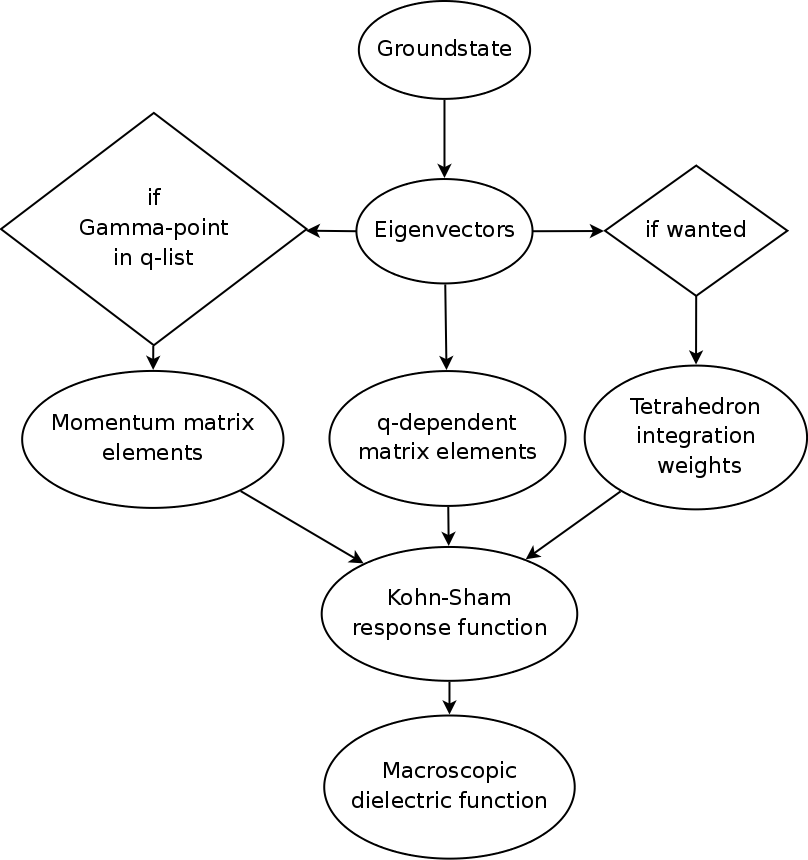
\includegraphics[height=1.65in,width=1.70in,viewport=0 0 1200 1300,clip]{Figures/lr-TDDFT_flowchart.png}
%\caption{\textrm{\tiny Flow diagram sketching the solution of the Bethe-Salpeter equation in practice.}}%(与文献\cite{EPJB33-47_2003}图1对比)
\label{lr-DFT-flowchart}
\end{figure}
}

\frame
{
	\frametitle{\textrm{TD-DFT}与\textrm{BSE}}
\begin{figure}[h!]
\centering
\vspace{-50pt}
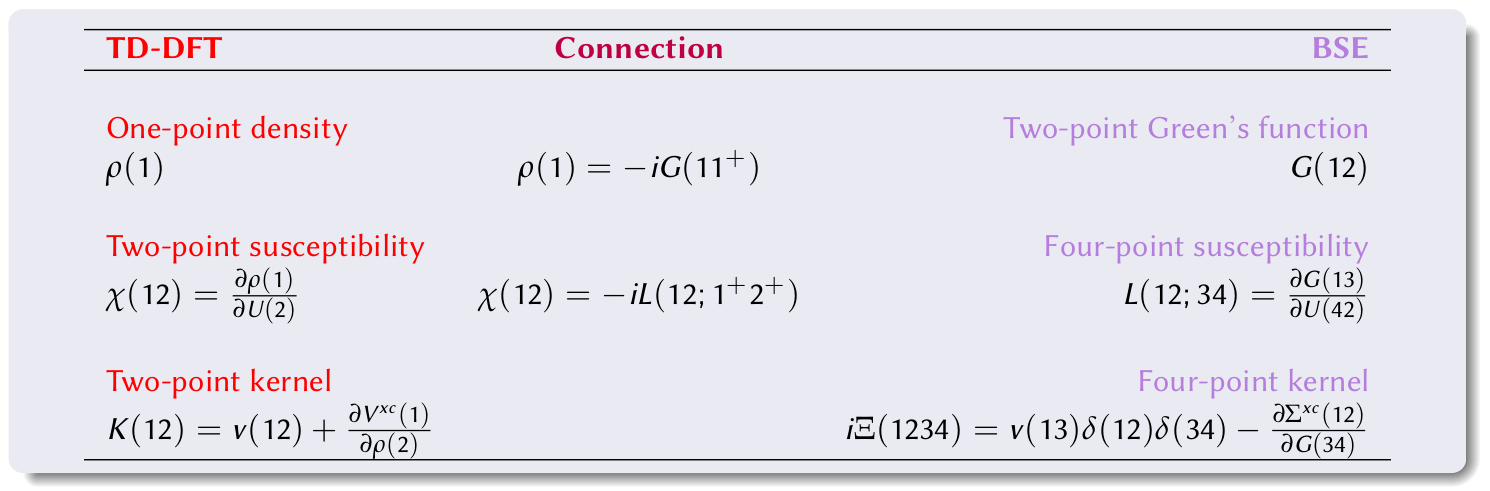
\includegraphics[height=2.05in,width=4.00in,viewport=50 0 1450 730,clip]{Figures/DFT_GW_BSE-compare.png}
%\caption{\textrm{\tiny Flow diagram sketching the solution of the Bethe-Salpeter equation in practice.}}%(与文献\cite{EPJB33-47_2003}图1对比)
\label{DFTGW-BSE_compare}
\end{figure}
\begin{itemize}
	\item \textrm{BSE}计算电子-空穴激发能精度较高,但计算量可观(须计算大量多中心积分)\\
		擅长处理周期体系
	\item \textrm{TD-DFT}通过线性响应计算激发态,灵活方便,计算量较小\\
		适合处理有限体系,拙于处理周期体系
\end{itemize}
}

\section{动力学平均场理论}
\frame
{
	\frametitle{电子强关联现象}
	有很多重要的物理现象都与电子强关联有关
	\begin{itemize}
		\item \textrm{Mott}绝缘体:\\
			过渡金属氧化物\textrm{(Transition metal oxides)}:~如~\textrm{\ch{V2O3}}
		\item \textrm{Kondo}效应\\
			稀磁合金中出现的磁性杂质-非磁性宿主金属之间的对抗引起的低温反常输运行为(电阻)
		\item 重\textrm{fermion}行为\\
			含有~$f$-电子的镧系或者锕系金属间化合物,有效质量比自由电子大$2\sim3$数量级:~如~\textrm{\ch{CeAl3}}
		\item 高温超导\textrm{(High-temperature Superconductivity)}\\
			钇钡铜氧$(\mathrm{YBa}_2\mathrm{Cu}_3\mathrm{O}_{7-x})$、铁基超导体
	\end{itemize}
	电子强关联:~独立粒子图像失效,\textrm{DFT}无法描述准确电子能带结构
}

\frame
{
	\frametitle{电子相关与能带结构}
\begin{figure}[h!]
\centering
\vspace{-12pt}
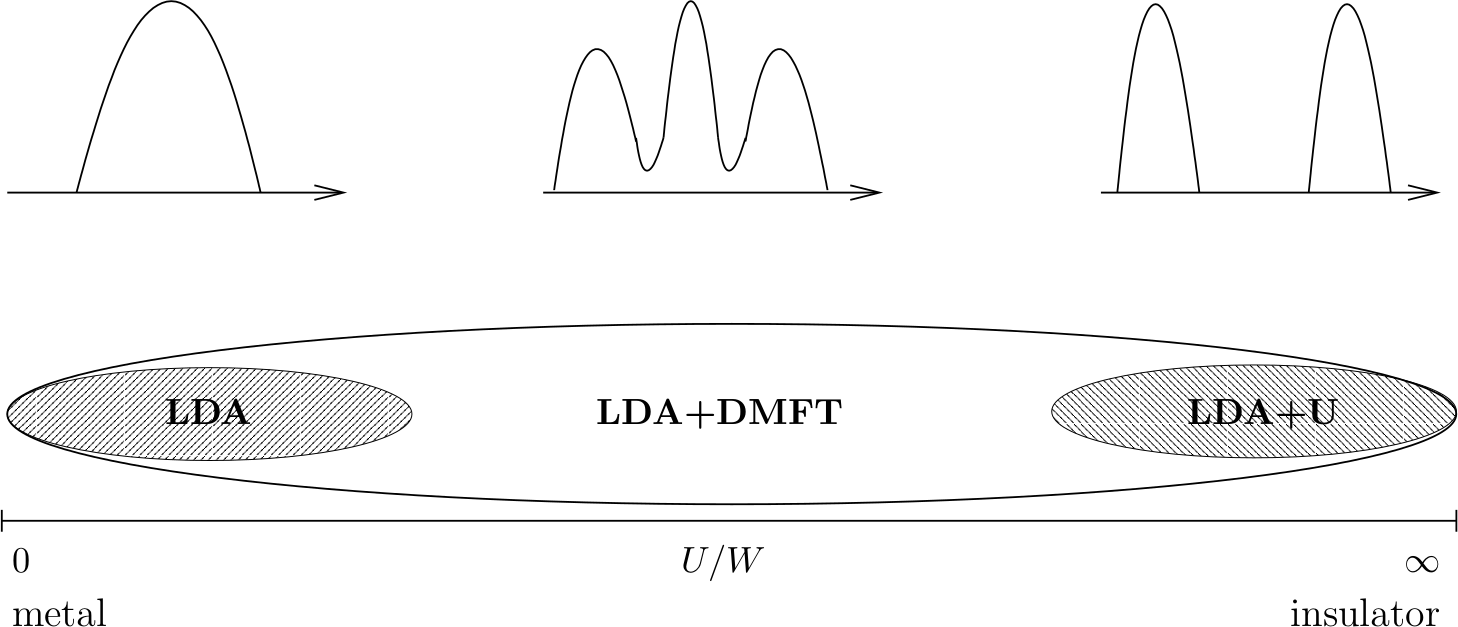
\includegraphics[height=2.5in,width=4.00in,viewport=0 0 1680 1000,clip]{Figures/DFT-DMFT-compare.png}
\caption{\textrm{\tiny The schematic diagram of electron-structure from DFT, DMFT and DFT+$U$.}}%(与文献\cite{EPJB33-47_2003}图1对比)
\label{DFT-DMFT-Hubbard}
\end{figure}
}

\frame
{
	\frametitle{\textrm{Hubbard}模型}
\begin{minipage}[b]{0.58\linewidth}
	\begin{displaymath}
		\begin{aligned}
			H=&\textcolor{cyan}{\varepsilon_d}\sum_{i,\sigma}c_{i\sigma}^{\dag}c_{j\sigma}-\sum_{\langle ij\rangle,\sigma=\uparrow,\downarrow}\underbrace{t_{ij}c_{i\sigma}^{\dag}c_{j\sigma}}_{\fontsize{6.2pt}{4.2pt}\selectfont{\textcolor{purple}{\mathrm{Kinetic~term}}}}\\
			&+\underbrace{\textcolor{blue}{U}n_{i\uparrow}n_{i\downarrow}}_{\fontsize{6.2pt}{4.2pt}\selectfont{\textcolor{purple}{\mathrm{Interaction~aterm}}}}~_{\fontsize{3.2pt}{2.2pt}\selectfont{\Longleftarrow\mathrm{(Coulomb)~\textcolor{blue}{U}>0}}} \\
			n_{i\sigma}\equiv&c_{i\sigma}^{\dag}c_{i\sigma}\\
		\end{aligned}
	\end{displaymath}
			{\fontsize{7.2pt}{5.2pt}\selectfont{\textrm{Doping~(number~of~charge)}
			\begin{displaymath}
				\delta=1-\langle n_{\uparrow}+n_{\downarrow}\rangle
			\end{displaymath}}}
\end{minipage}
\hfill
\begin{minipage}[t]{0.40\linewidth}
\begin{figure}[h!]
\centering
\vspace{-120pt}
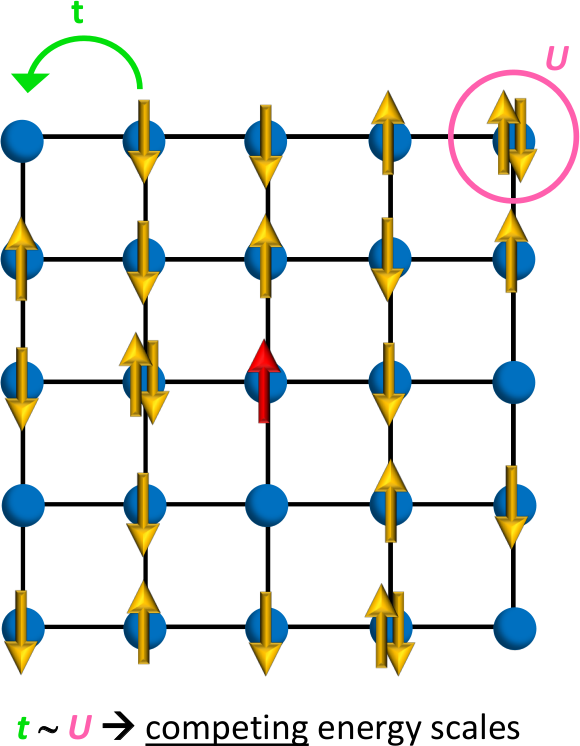
\includegraphics[height=2.0in,width=1.65in,viewport=0 0 600 750,clip]{Figures/Hubbard_U-t.png}
%\caption{\textrm{\tiny Flow diagram sketching the solution of the Bethe-Salpeter equation in practice.}}%(与文献\cite{EPJB33-47_2003}图1对比)
\label{Hubbard-U}
\end{figure}
\end{minipage}
\vspace*{-25pt}
\begin{itemize}
	\item 半充满:~1~电子/格点平均:~$\delta=0$
	\item $U/t$小:~\textrm{Fermi}液体
	\item $t=0$:~原子极限
	\item \textcolor{red}{$U/t$是中等耦合:~?}
\end{itemize}
}

\frame
{
	\frametitle{\textrm{Hubbard}模型描述的\textrm{Mott}转变}
\begin{minipage}[b]{0.42\linewidth}
	\hspace{45pt} \textrm{Bethe}~晶格
\begin{figure}[h!]
\centering
\vspace{-5pt}
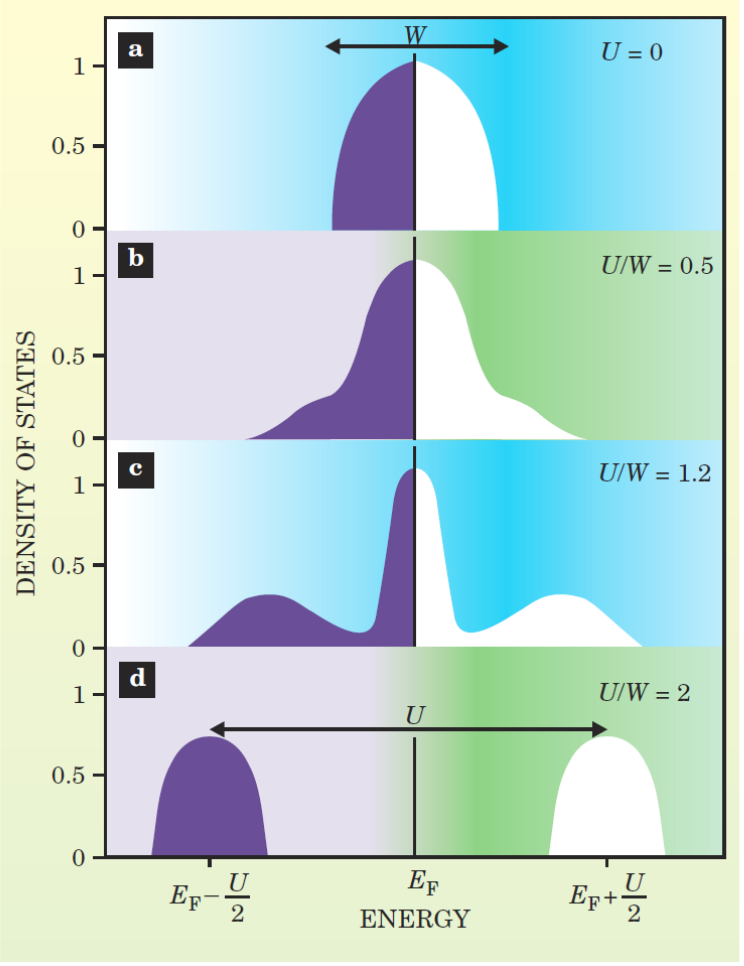
\includegraphics[height=2.1in,width=2.00in,viewport=0 0 800 950,clip]{Figures/Hubbard_U-W.png}
\caption{\textrm{\tiny Mott transition within the Hubbard model.引自文献\cite{PT57-53_2004}}}%}}%(图1对比)
\label{Mott_Hubbard}
\end{figure}
\end{minipage}
\hfill
\begin{minipage}[t]{0.56\linewidth}
	\vspace*{-2.58in}
	\begin{itemize}
		\setlength{\itemsep}{14pt}
		\item \textrm{a}:~自由电子气
		\item \textrm{b}:~近理想金属:~\textrm{Fermi}液体理论(准粒子图像)有效
		\item \textrm{c}:~强关联金属:~出现典型的三峰结构({\fontsize{7.2pt}{5.2pt}\selectfont{\textrm{Hubbard}能带+准粒子峰}})
		\item \textrm{d}:~\textrm{Mott}绝缘体:~准粒子峰消失,出现\textrm{Mott}金属-绝缘体转变
	\end{itemize}
\end{minipage}
}

\frame
{
	\frametitle{超越单粒子图像}
\begin{minipage}[b]{0.49\linewidth}
	巡游电子~\textrm{vs}~能带 
\begin{figure}[h!]
\centering
\vspace{-5pt}
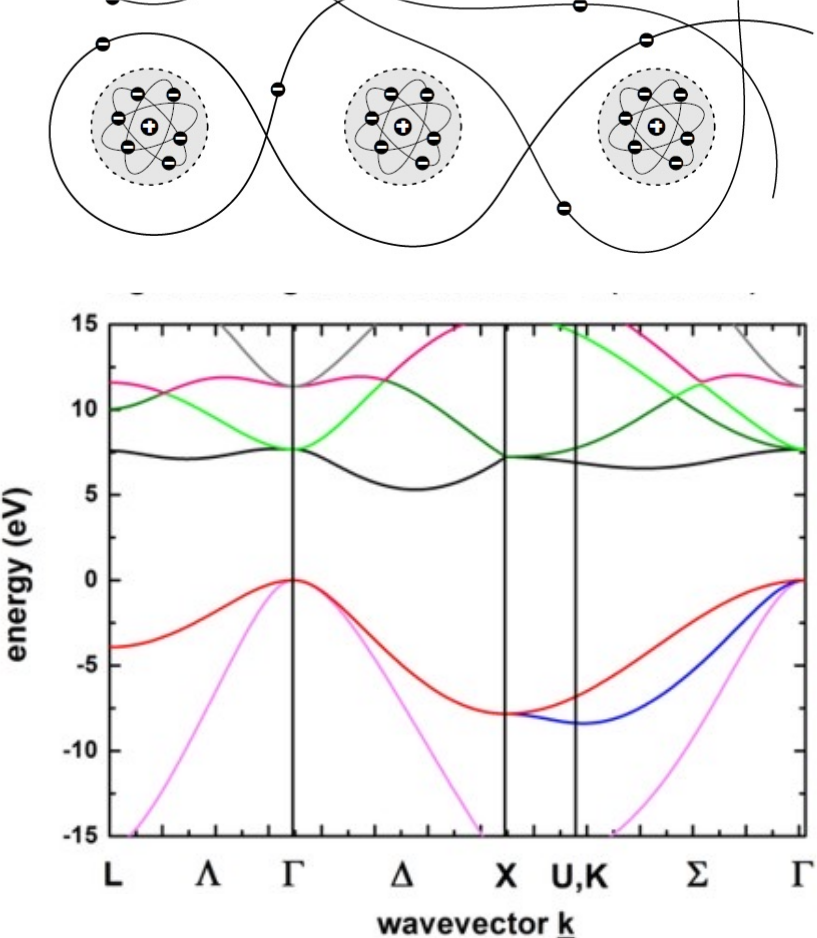
\includegraphics[height=1.7in,width=1.45in,viewport=0 0 860 950,clip]{Figures/Itinerant_electrons-bands.png}
%\caption{\textrm{\tiny The schematic diagram of electron-structure from DFT, DMFT and DFT+$U$.}}%(与文献\cite{EPJB33-47_2003}图1对比)
\label{Itinerant-band}
\end{figure}
{\fontsize{7.2pt}{6.2pt}\selectfont{
\begin{itemize}
	\item 非简并的基态
	\item 单\textrm{Slater}行列式
\end{itemize}}}
\end{minipage}
\hfill
\begin{minipage}[b]{0.49\linewidth}
	局域电子~\textrm{vs}~多重态(精细结构)
\begin{figure}[h!]
\centering
\vspace{-5pt}
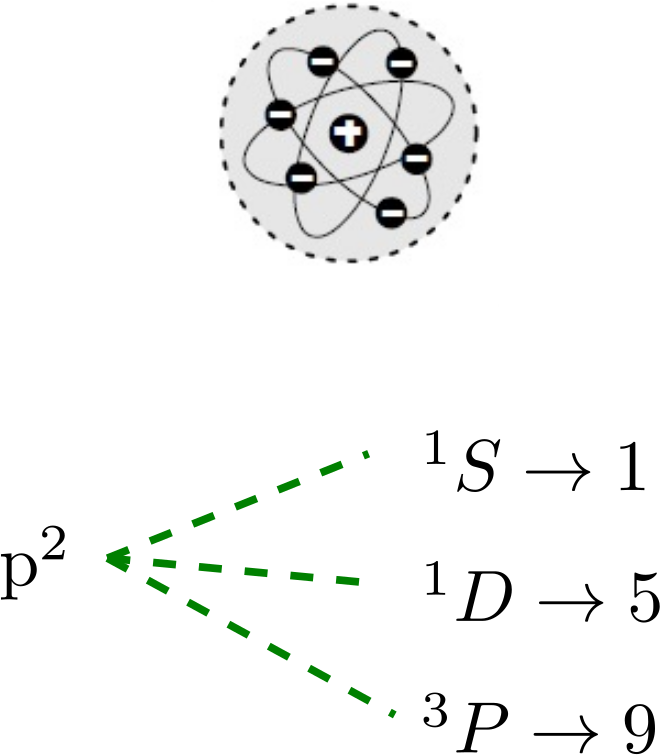
\includegraphics[height=1.7in,width=1.50in,viewport=0 0 700 770,clip]{Figures/Localized_electrons-multiplets.png}
%\caption{\textrm{\tiny The schematic diagram of electron-structure from DFT, DMFT and DFT+$U$.}}%(与文献\cite{EPJB33-47_2003}图1对比)
\label{Localized-multiplets}
\end{figure}
{\fontsize{7.2pt}{6.2pt}\selectfont{
\begin{itemize}
	\item (近)简并的基态
	\item 多个\textrm{Slater}行列式的线性组合
\end{itemize}}}
\end{minipage}
\begin{itemize}
\vspace{-12pt}
	\item 含有开壳层的$d$和$f$电子体系是介于局域态和巡游态之间
	\item 超越单电子图像才能维持多重态结构
\end{itemize}
}

\frame
{
	\frametitle{\textrm{Ising}模型的\textrm{Weiss}平均场}
	\begin{itemize}
		\item 杂质:~平均场效应下包含电子相关效应的单个格点
		\item 浴:~模仿废弃的晶格位效果的电子海洋
		\item 杂化:~耦合$b/w$杂质和浴,用$\Delta(\omega)=\frac{V^2}{[\omega-(\varepsilon-\mu)]}$对浴态全部求和来描述
		\item 杂质\textrm{Green's function}$G(\omega)$:~杂质问题的\textrm{Green's function}
		\item 浴\textrm{Green's function}$\mathcal{G}(\omega)$:~杂质问题的无相互作用\textrm{Green's function}
		\item 晶格\textrm{Green's function}$G(\vec k,\omega)$:~特定$\vec k$点上的\textrm{Green's function}
		\item 局域\textrm{Green's function}$G_{ii}(\omega)$:~全部$\vec k$点的晶格\textrm{Green's function}的求和
		\item 自能$\Sigma(\omega)$:~一个粒子的能量其实部对应谱学中相互作用诱导引起的移动,虚部对应谱学展宽
	\end{itemize}
}

\frame
{
	\frametitle{经典平均场理论}
%	动力学平均场理论\textrm{(Dynamic Mean Field Theory, DMFT)}
%	是一种确定强关联材料电子结构的方法。在这种材料中,用于密度泛函理论和通常的能带结构计算的独立电子近似失效了。动力学平均场理论是对电子之间局部相互作用的非微扰处理,它在近自由电子气极限和凝聚态物理学的原子极限之间架起了桥梁。
	\begin{itemize}
		\item \textrm{Hartree-Fock}理论\\
			每个电子都在其它运动电子构成的平均场中运动,感受的是其它电子瞬时作用的平均值
		\item \textrm{Weiss}平均场理论
			\begin{itemize}
				\item 铁磁态的\textrm{CUrie-Weiss}定律:~经典的自旋体系(\textrm{Ising}模型),每个格点处自旋感受到的磁场源于所有其余各格点自旋的平均
				\item 当自旋体系的维度$d\rightarrow\infty$时,理论趋于精确(受控近似)
			\end{itemize}
\end{itemize}
}

\frame
{\frametitle{\textrm{Ising}模型的\textrm{Weiss}平均场}
\begin{itemize}
	\item \textrm{Ising}模型
\begin{figure}[h!]
\centering
\vspace{-15pt}
%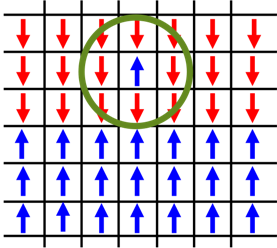
\includegraphics[height=1.0in,width=1.15in,viewport=0 0 130 120,clip]{Figures/MC-Ising-model_2.png}
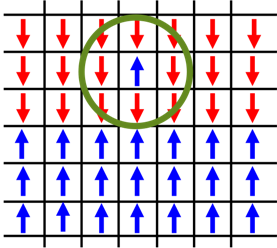
\includegraphics[height=0.5in,width=0.65in,viewport=0 0 130 120,clip]{Figures/MC-Ising-model_2.png}
%\caption{\textrm{\tiny The schematic diagram of electron-structure from DFT, DMFT and DFT+$U$.}}%(与文献\cite{EPJB33-47_2003}图1对比)
\label{Ising-Model}
\end{figure}
\begin{displaymath}
	H=-\frac J2\sum_{\langle\mathbf{R}_i\mathbf{R}_j\rangle}S_iS_j-h\sum_{\mathbf{R}_i}S_i
\end{displaymath}
{\fontsize{7.2pt}{6.2pt}\selectfont{这里$S=\pm1$;~$h$是均匀外场;~$J>0$表示铁磁耦合}}
\item 引入\textrm{Weiss}平均场
	\begin{displaymath}
		\begin{aligned}
			H_{\mathrm{MF}}=&-\textcolor{red}{h_{\mathrm{MF}}}\sum_iS_i\\
			\textcolor{red}{h_{\mathrm{MF}}}=&J\sum_{\mathbf{R}_j}^{(i)}\langle S_j\rangle+h=\textcolor{blue}{Z}J\langle S\rangle+h\\
			&\mbox{\fontsize{6.2pt}{6.2pt}\selectfont{这里对$\mathbf{R}_j$的求和遍历格点$i$的全部最紧邻点}}
		\end{aligned}
	\end{displaymath}
	{\fontsize{8.2pt}{6.2pt}\selectfont{$Z$:~最近邻格点数(维度数)}}
\end{itemize}
}

\frame
{\frametitle{\textrm{Ising}模型的\textrm{Weiss}平均场}
\textrm{Curie-Weiss}自洽方程为
\begin{displaymath}
	\langle S\rangle=\tanh\left[\frac{ZJ\langle S\rangle+h}{k_{\mathrm{B}}T}\right]
\end{displaymath}
\begin{minipage}[t]{0.39\linewidth}
	\vspace*{-2in}
\begin{itemize}
		\setlength{\itemsep}{14pt}
	\item 有限温度下,顺磁态和铁磁态间存在相变
	\item 当维度$Z\rightarrow\infty$,自洽方程的解是精确的
	\item $J$的取值:~当$J^{\ast}$是常数,$J=J^{\ast}/Z$
\end{itemize}
\end{minipage}
\hfill
\begin{minipage}[b]{0.59\linewidth}
\begin{figure}[h!]
\centering
%\vspace{-2pt}
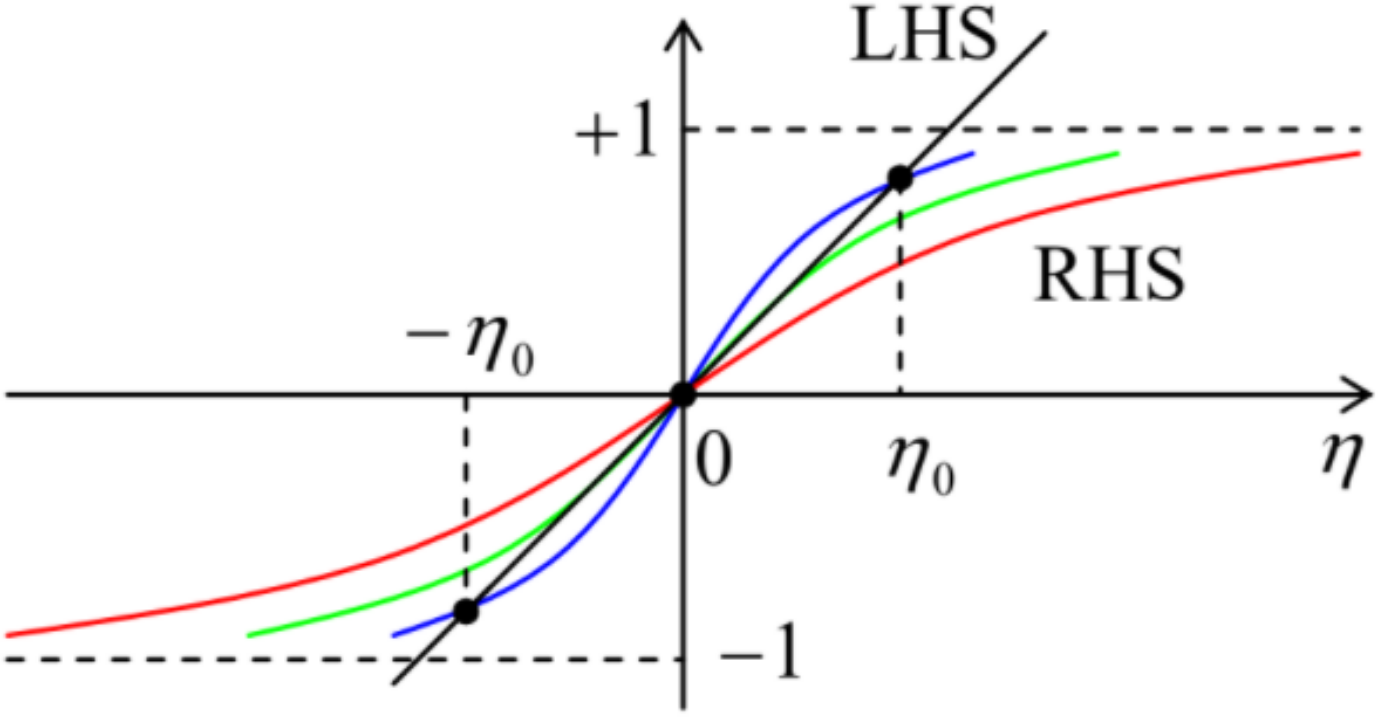
\includegraphics[height=1.2in,width=2.35in,viewport=0 0 1380 720,clip]{Figures/Ferromagnetic_phase_transition-in-Weiss_molecular-field-theory.png}
\caption{\textrm{\tiny .The ferromagnetic phase transition in Weiss' molecular-field theory: two sides of Equation self-consistent equation sketched as functions of $\eta$ for three different temperatures:~above T (red), below T (blue), and equal to T (green).}}%(与文献\cite{EPJB33-47_2003}图1对比)
\label{Ising-Model_Ferromagnetic_phase_transition}
\end{figure}
\end{minipage}
}

\frame
{
	\frametitle{$Z\rightarrow\infty$极限}
\begin{minipage}[b]{0.25\linewidth}
\begin{figure}[h!]
\centering
%\vspace{-2pt}
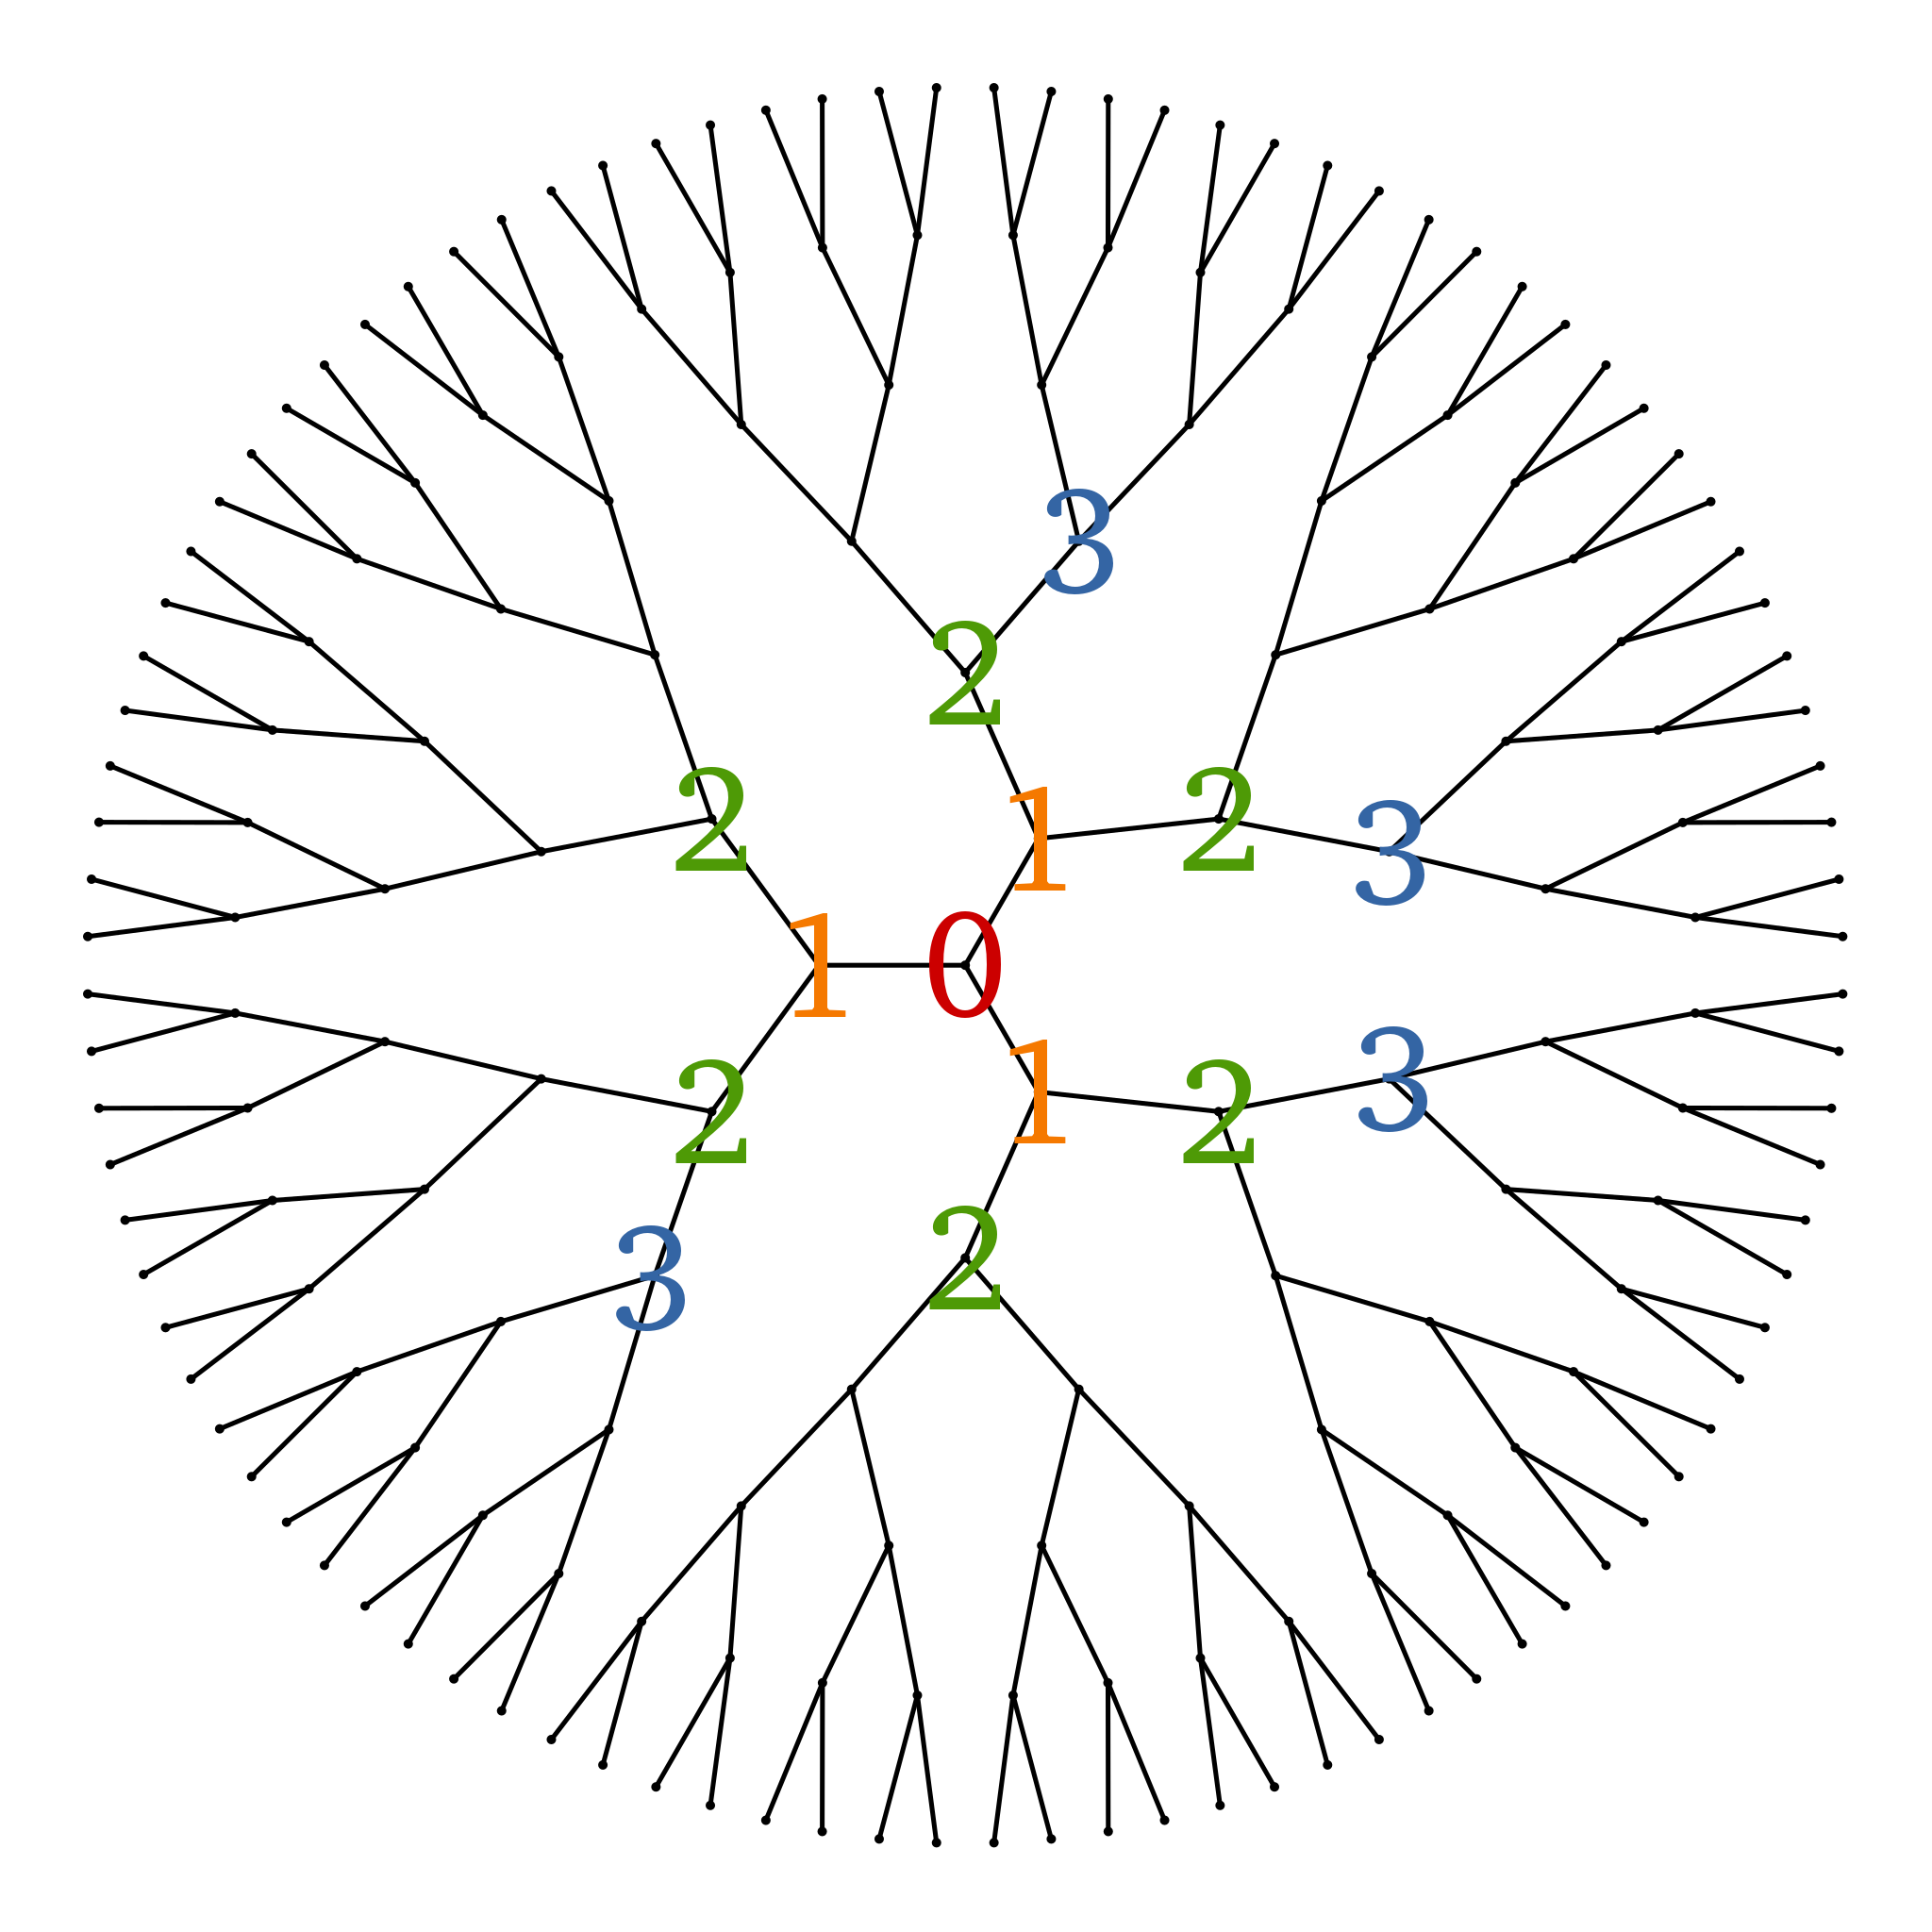
\includegraphics[height=1.0in,width=1.05in,viewport=0 0 1980 1980,clip]{Figures/Bethe-Lattice-Ising_Model.png}
%\caption{\textrm{\tiny .The ferromagnetic phase transition in Weiss' molecular-field theory: two sides of Equation self-consistent equation sketched as functions of $\eta$ for three different temperatures:~above T (red), below T (blue), and equal to T (green).}}%(与文献\cite{EPJB33-47_2003}图1对比)
\label{Bethe-Lattice_Ising-Model_Limit-1}
\end{figure}
\end{minipage}
\hfill
\begin{minipage}[t]{0.14\linewidth}
	\vspace{-1in} 
	\begin{displaymath}
		\xrightarrow[Z\rightarrow\infty]{d\rightarrow\infty}
	\end{displaymath}
\end{minipage}
\hfill
\begin{minipage}[b]{0.55\linewidth}
\begin{figure}[h!]
\centering
%\vspace{-2pt}
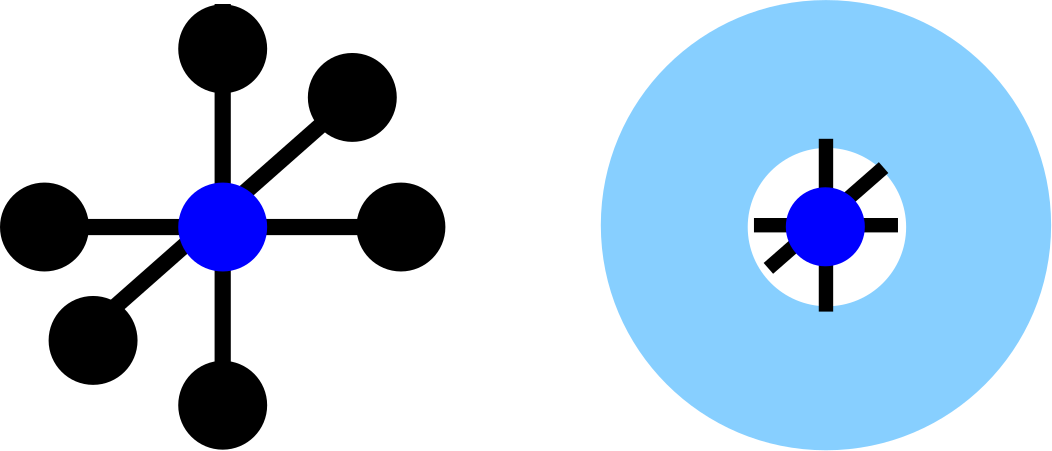
\includegraphics[height=1.0in,width=2.35in,viewport=0 0 1050 455,clip]{Figures/Bethe-Lattice.png}
%\caption{\textrm{\tiny .The ferromagnetic phase transition in Weiss' molecular-field theory: two sides of Equation self-consistent equation sketched as functions of $\eta$ for three different temperatures:~above T (red), below T (blue), and equal to T (green).}}%(与文献\cite{EPJB33-47_2003}图1对比)
\label{Bethe-Lattice_Ising-Model_Limit-2}
\end{figure}
\end{minipage}
\begin{itemize}
	\item 对于给定的格点$i$,当$d\rightarrow\infty$,单个最紧邻自旋贡献不再重要,取平均值为宜
	\item 晶格问题也约化为单个格点的平均场问题
\end{itemize}
}

\frame
{
	\frametitle{\textrm{Ising}模型的\textrm{Weiss}平均场}
	\begin{itemize}
		\item 杂质:~平均场效应下包含电子相关效应的单个格点
		\item 浴:~模仿废弃的晶格位效果的电子海洋
		\item 杂化:~耦合$b/w$杂质和浴,用$\Delta(\omega)=\frac{V^2}{[\omega-(\varepsilon-\mu)]}$对浴态全部求和来描述
		\item 杂质\textrm{Green's function}$G(\omega)$:~杂质问题的\textrm{Green's function}
		\item 浴\textrm{Green's function}$\mathcal{G}(\omega)$:~杂质问题的无相互作用\textrm{Green's function}
		\item 晶格\textrm{Green's function}$G(\vec k,\omega)$:~特定$\vec k$点上的\textrm{Green's function}
		\item 局域\textrm{Green's function}$G_{ii}(\omega)$:~全部$\vec k$点的晶格\textrm{Green's function}的求和
		\item 自能$\Sigma(\omega)$:~一个粒子的能量其实部对应谱学中相互作用诱导引起的移动,虚部对应谱学展宽
	\end{itemize}
}

\frame
{
	\frametitle{\textrm{Anderson}模型}
	\textrm{Anderson}模型
	\begin{displaymath}
		\begin{aligned}
			H_{\mathrm{A}}=&\underbrace{\sum_{\vec k}\sum_{\sigma}\varepsilon_{\vec k}n_{\vec k\sigma}}_{\textcolor{blue}{\mathrm{metal}}}+\underbrace{\sum_{\sigma}\varepsilon_fn_{f\uparrow}n_{f\downarrow}+Un_{f\uparrow}n_{f\downarrow}}_{\textcolor{magenta}{\mathrm{impurity}}}\\
			+&\underbrace{\sum_{\vec k}\sum_{\sigma}\big[V_{\vec k}c_{\vec k\sigma}^{\dag}c_{f\sigma}+h.c.\big]}_{\textcolor{purple}{\mathrm{hybridization}}}
		\end{aligned}
	\end{displaymath}
	\textrm{Kondo}区域:~$n_f\sim1$

	通过正则变换\textrm{(Schrieffer-Wolff~变换)}成为\textrm{Kondo}模型
	\begin{displaymath}
		H_{\mathrm{K}}=\sum_{\vec k}\sum_{\sigma}\varepsilon_{\vec k}n_{\vec k\sigma}+\Gamma\mathbf{S}_f\cdot\mathbf{S}_c(\mathbf{0})=H_0+H_{\Gamma}
	\end{displaymath}
	\begin{displaymath}
		\Gamma\sim -2|V_{k_{\mathrm{F}}}|^2\left[\frac1{\varepsilon_f-\frac1{\varepsilon_f+U}}\right]>0
	\end{displaymath}
反铁磁耦合
}

\frame
{
	\frametitle{动力学平均场}
	晶格中的多体相互作用电子态
	\begin{itemize}
		\item 类局域态电子:~在每个格点上形成多重态
		\item 类巡游态电子:~电子在格点间跳跃
	\end{itemize}
\begin{figure}[h!]
\centering
\vspace{-5pt}
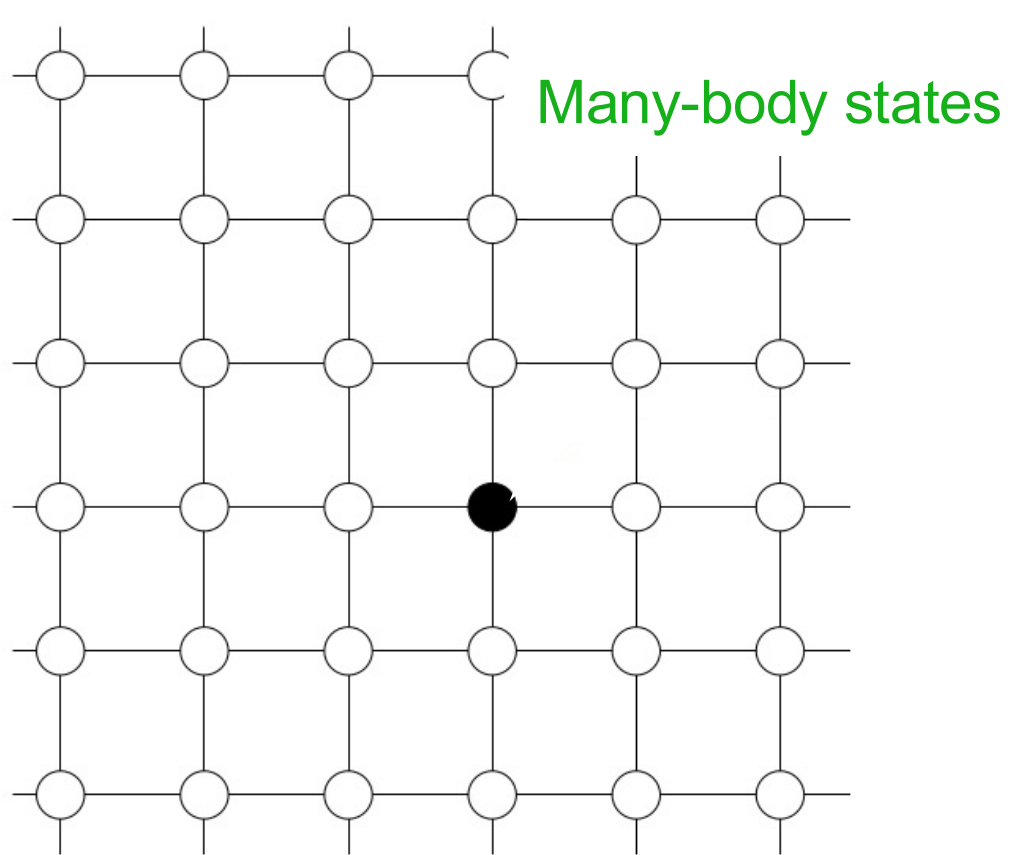
\includegraphics[height=1.5in,width=1.80in,viewport=0 0 970 820,clip]{Figures/Lattice_Many-body-states.png}
%\caption{\textrm{\tiny The schematic diagram of electron-structure from DFT, DMFT and DFT+$U$.}}%(与文献\cite{EPJB33-47_2003}图1对比)
\label{Localized-multiplets}
\end{figure}
	将量子多电子问题转成等效平均场中的量子杂质问题
	\begin{displaymath}
		S_{\mathrm{eff}}=-\int_0^{\beta}\underbrace{\mathrm{d}\tau\mathrm{d}\tau^{\prime}\mathrm{d}_{\sigma\sigma^{\prime}}\mathcal{G}_0^{-1}(\tau,\tau^{\prime})\mathrm{d}_{\sigma\sigma^{\prime}}(\tau^{\prime})}_{\textcolor{red}{{\fontsize{6.2pt}{4.2pt}\selectfont{Electron~hopping}}}}+\int\mathrm{d}\tau\underbrace{Un_{0\uparrow}(\tau)n_{0\downarrow}(\tau)}_{\textcolor{green}{{\fontsize{6.2pt}{4.2pt}\selectfont{Multiplets}}}}
	\end{displaymath}
	局域近似,不存在平移周期(与$\vec k$无关),但可以存在非局域延展
}

\frame
{
	\frametitle{无限维的\textrm{Hubbard}模型}
	对于非相互作用部分
	\begin{displaymath}
		H_0=-t\sum_{\langle i,j\rangle,\sigma}c_{i\sigma}c_{j\sigma}^{\dag}=\sum_{\vec k\sigma}\varepsilon_{\vec k}n_{\vec k\sigma}
	\end{displaymath}
	对于超立方晶格
	\begin{displaymath}
		\varepsilon=-2t\sum_{i}^d\cos(k_ia)
	\end{displaymath}
	非相互作用的态密度
	\begin{displaymath}
		D_0(E)=2\sum_{\vec k}\delta(E-\varepsilon_{\vec k})\xrightarrow[]{d\rightarrow\infty}\frac1{t\sqrt{\pi d}}\mathrm{exp}\left[-\left(\frac{E}{2t\sqrt{(d)}}\right)^2\right]
	\end{displaymath}
	对于$d\rightarrow\infty$要得到非平凡解,$t$的取值为
	\begin{displaymath}
		t=\frac{t^{\ast}}{\sqrt d}\quad t^{\ast}=\mathrm{const}
	\end{displaymath}
}

\frame
{
	\frametitle{$d\rightarrow\infty$}
	\begin{displaymath}
		H=-\frac{t^{\ast}}{\sqrt d}\sum_{\langle i,j\rangle,\sigma}c_{i\sigma}c_{j\sigma}^{\dag}+U\sum_in_{\i\uparrow}n_{i\downarrow}
	\end{displaymath}
	当$d\rightarrow\infty$,有$G_{\langle i,j\rangle,\sigma}(\omega)\sim\mathcal{O}\left(\frac1{\sqrt d}\right)$
	粒子是非局域的
	\begin{displaymath}
		\sum_j|G_{\langle i,j\rangle,\sigma}|^2\sim\mathcal{O}(1)
	\end{displaymath}
	合理的自能是局域的
	\begin{displaymath}
		\Sigma_{ij}(\omega)=\Sigma_{ii}(\omega)\delta_{ij}
	\end{displaymath}
}

\frame
{
	\frametitle{晶格格点约化为单格点}
	体系用量子力学作用算符描述
	\begin{displaymath}
		\begin{aligned}
			S=&\int_0^{\beta}\mathrm{d}\tau\left(\sum_{i\sigma}c_{i\sigma}\partial_{\tau}c_{i\sigma}^{\dag}-t\sum_{\langle ij\rangle,\sigma}c_{i\sigma}c_{i\sigma}^{\dag}-\mu\sum_{i\sigma}n_{i\sigma}+U\sum_in_{i\uparrow}n_{i\downarrow}\right)\\
			\beta=&k_{\mathrm{B}}T\qquad\mbox{\fontsize{6.2pt}{6.2pt}\selectfont{这里$c_{i\sigma}$和$c_{i\sigma}^{\dag}$称为\textrm{Grassmann~变量}}}
		\end{aligned}
	\end{displaymath}
\begin{minipage}[b]{0.59\linewidth}
	\begin{displaymath}
		\mathrm{e}^{-S_{\mathrm{eff}}[c_0,c_0^{\dag}]}=\int\prod_{i\neq 0,\sigma}Dc_{i\sigma}^{\dag}Dc_{i\sigma}\mathrm{e}^{-S[c_{i\sigma},c_{i\sigma}^{\dag}]}
	\end{displaymath}
定义配分函数
\begin{displaymath}
	Z_{\mathrm{eff}}=\int Dc_{0\sigma}^{\dag}Dc_{0\sigma}\mathrm{e}^{-S[c_0,c_0^{\dag}]} 
\end{displaymath}
定义局域传播子
\begin{displaymath}
	G_{\mathrm{eff}}=\int Dc_{0\sigma}^{\dag}Dc_{0\sigma}c_{0\sigma}(\mathrm{i}\omega_n)c_{0\sigma}^{\dag}(\mathrm{i}\omega_n)\mathrm{e}^{-S_{\mathrm{eff}}[c_0,c_0^{\dag}]}
\end{displaymath}
\end{minipage}
\hfill
\begin{minipage}[b]{0.39\linewidth}
\begin{figure}[h!]
\centering
\vspace{-20pt}
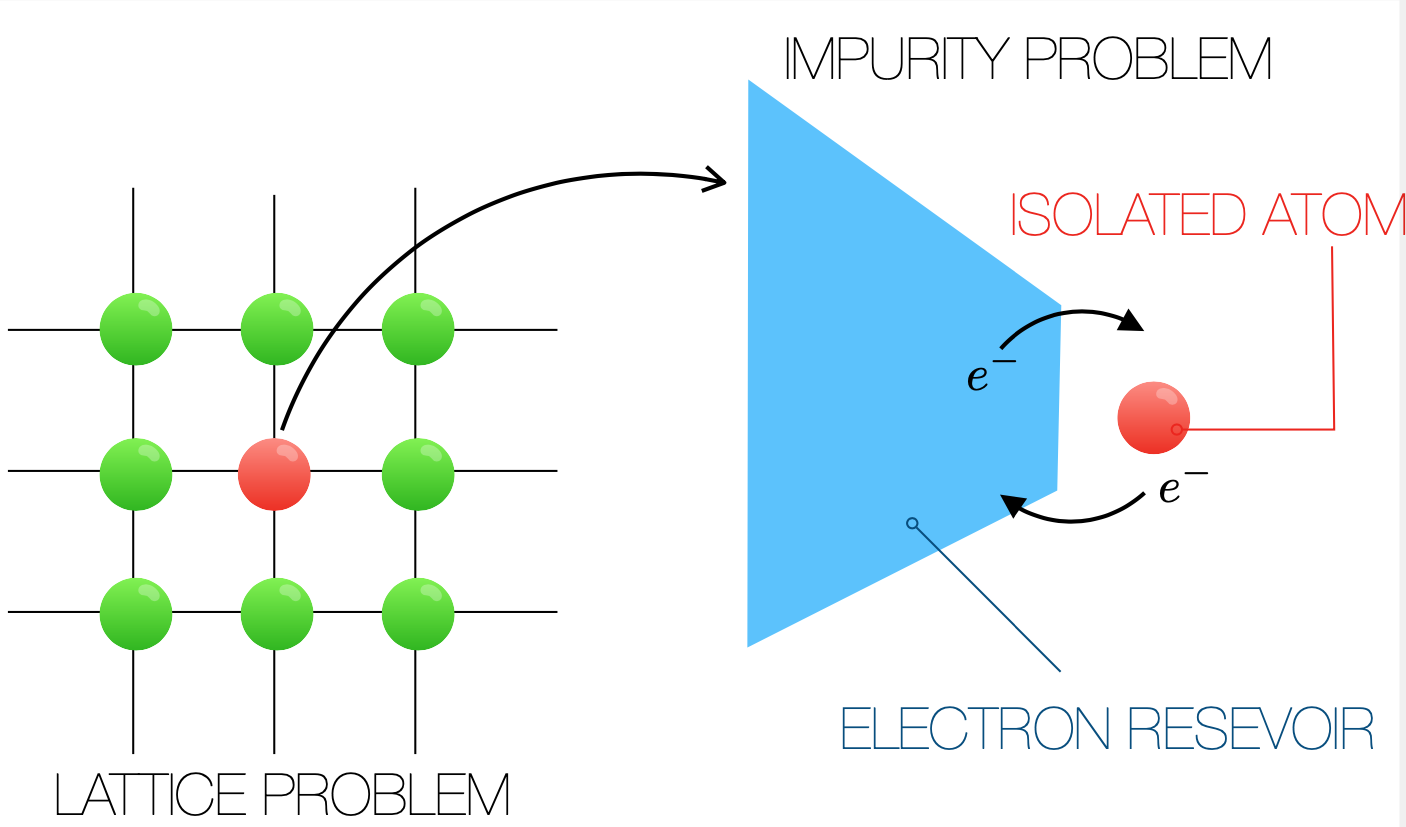
\includegraphics[height=1.0in,width=1.85in,viewport=0 0 750 455,clip]{Figures/Dmft_lattice-atom.png}
%\caption{\textrm{\tiny .The ferromagnetic phase transition in Weiss' molecular-field theory: two sides of Equation self-consistent equation sketched as functions of $\eta$ for three different temperatures:~above T (red), below T (blue), and equal to T (green).}}%(与文献\cite{EPJB33-47_2003}图1对比)
\label{Dmft_lattice-atom.}
\end{figure}
\end{minipage}
}

\frame
{
	\frametitle{\textrm{DMFT}方程}
	当$d\rightarrow\infty$,简化$S_{\mathrm{eff}}$
	\begin{displaymath}
		S_{\mathrm{eff}}=\int_0^{\beta}\mathrm{d}\tau\int_0^{\beta}\mathrm{d}\tau^{\prime}(c_{0\sigma}^{\dag})\mathcal{G}^{-1}(\tau-\tau^{\prime})c_{0\sigma}(\tau^{\prime})+U\int_0^{\beta}\mathrm{d}\tau n_{0\uparrow}(\tau)n_{0\downarrow}(\tau)
	\end{displaymath}
	其中\textrm{bath~Green's function}为
	\begin{displaymath}
		\begin{aligned}
			\mathcal{G}^{-1}(\mathrm{i}\omega_n)=&\Sigma(\mathrm{i}\omega_n)+\left[\sum_{\vec k}\frac1{\mathrm{i}\omega_n+\mu-\varepsilon_{\vec k}-\Sigma_{\mathrm{i}\omega_n}}\right]^{-1}\\
			=&\Sigma(\mathrm{i}\omega_n)+\big[\sum_{\vec k}G_{\vec k}(\mathrm{i}\omega_n)\big]^{-1}\\
			=&\Sigma(\mathrm{i}\omega_n)+G_{ii}^{-1}(\mathrm{i}\omega_n)
		\end{aligned}
	\end{displaymath}
	自洽条件为
	\begin{displaymath}
		G_{\mathrm{eff}}(\mathrm{i}\omega_n)=G_{ii}(\mathrm{i}\omega_n)
	\end{displaymath}
}

\frame
{
	\frametitle{动力学平均场的成效}
\begin{figure}[h!]
\centering
\vspace{-8pt}
\includegraphics[height=0.8in,width=2.65in,viewport=0 0 1450 470,clip]{Figures/The-Dmft-site_atom-embedded.png}
%\caption{\textrm{\tiny .The ferromagnetic phase transition in Weiss' molecular-field theory: two sides of Equation self-consistent equation sketched as functions of $\eta$ for three different temperatures:~above T (red), below T (blue), and equal to T (green).}}%(与文献\cite{EPJB33-47_2003}图1对比)
\label{Dmft_site_atom-embeddded}
\end{figure}
\begin{itemize}
	\item 晶格模型由等效的杂质模型代替,杂质与介质的作用通过自洽迭代确定
	\item 粒子的空间涨落被压制,但是局域的量子涨落则完全保留
\end{itemize}
\begin{figure}[h!]
\centering
\vspace{-6pt}
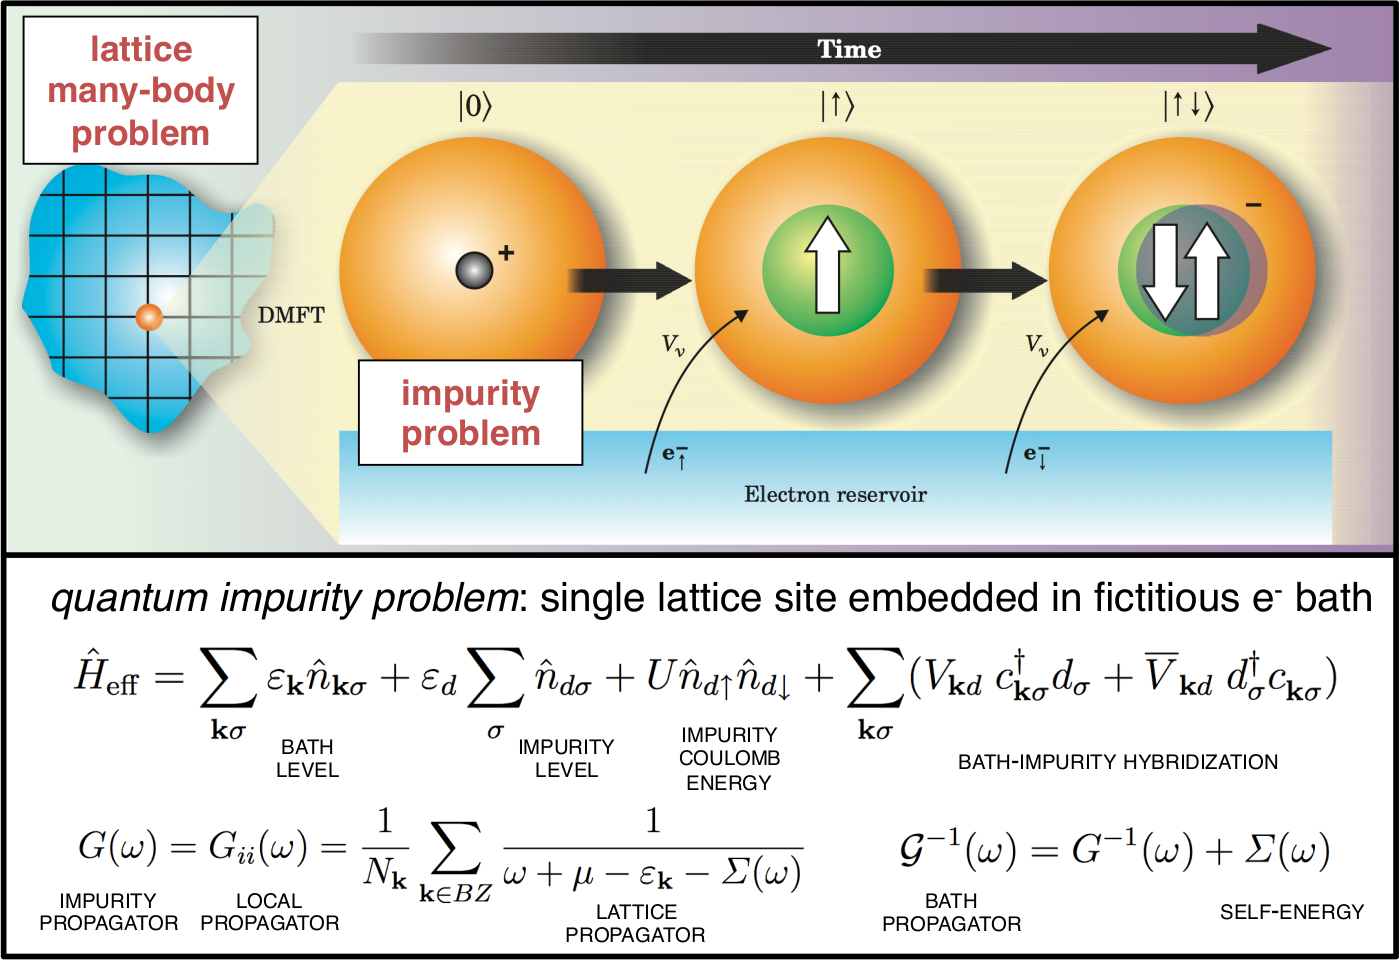
\includegraphics[height=1.35in,width=1.75in,viewport=0 0 1420 985,clip]{Figures/Quantum_impurity_problem.png}
%\caption{\textrm{\tiny .The ferromagnetic phase transition in Weiss' molecular-field theory: two sides of Equation self-consistent equation sketched as functions of $\eta$ for three different temperatures:~above T (red), below T (blue), and equal to T (green).}}%(与文献\cite{EPJB33-47_2003}图1对比)
\label{Qunatum_impurity_primble}
\end{figure}
}

\frame
{
	\frametitle{杂质求解器}
	将单格点问题映射为\textrm{Anderson}模型的单杂质点\textrm{(SIAM)}
	\begin{displaymath}
			H_{\mathrm{AM}}=\sum_{l\sigma}\tilde{\varepsilon}_la_{l\sigma}a_{l\sigma}^{\dag}-\mu\sum_{\sigma}c_{\sigma}c_{\sigma}^{\dag}+Un_{\uparrow}n_{\downarrow}+\sum_{l\sigma}V_l(c_{\sigma}a_{l\sigma}^{\dag}+a_{l\sigma}c_{\sigma}^{\dag})
	\end{displaymath}
	\textrm{Anderson}模型:~描述了一般金属中的磁性杂质

	对$a_l^{\dag}$和$a_l$积分,有
	\begin{displaymath}
		S_{\mathrm{eff}}=-\int_0^{\beta}\mathrm{d}\tau\int_0^{\beta}\mathrm{d}\tau^{\prime}\sum_{\sigma}c_{0\sigma}^{\dag}(\tau)\mathcal{G}^{-1}(\tau-\tau^{\prime})c_{0\sigma}(\tau^{\prime})+U\int_0^{\beta}\mathrm{d}\tau n_{0\uparrow}(\tau)n_{0\downarrow}(\tau)
	\end{displaymath}
这里
\begin{displaymath}
	\begin{aligned}
		\mathcal{G}_0^{-1}(\mathrm{i}\omega_n)=&\mathrm{i}\omega_n+\mu-\int_{-\infty}^{+\infty}\mathrm{d}\omega\frac{\Delta(\omega)}{\mathrm{i}\omega_n-\varepsilon}\\
		\Delta(\varepsilon)=&\sum_{l\sigma}V_l^2\delta(\varepsilon-\tilde{\varepsilon}_l)
	\end{aligned}
\end{displaymath}
}

\frame
{
	\frametitle{\textrm{DMFT}的计算流程}
\begin{figure}[h!]
\centering
\vspace{-2pt}
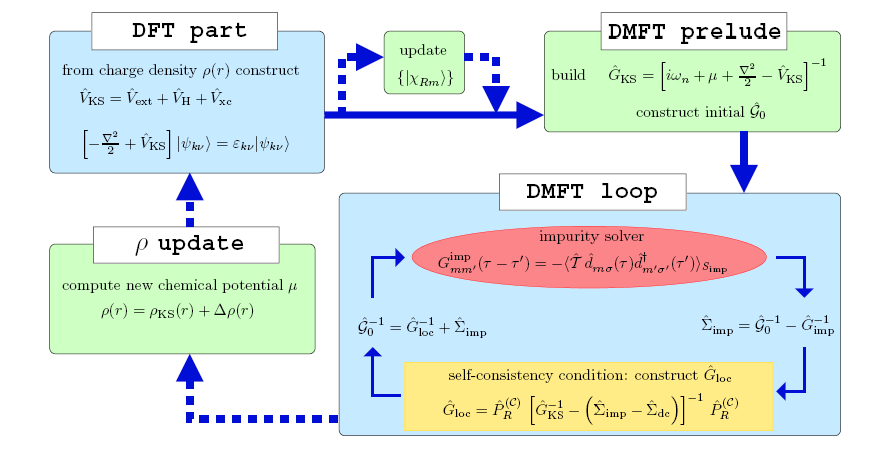
\includegraphics[height=2.4in,width=4.00in,viewport=0 0 780 420,clip]{Figures/DMFT_flowchart.png}
\caption{\textrm{\tiny The schematic diagram for a charge self-consistent DFT+DMFT loop.}}%(与文献\cite{EPJB33-47_2003}图1对比)
\label{DFT-DMFT-Flowchart}
\end{figure}
}
%\frame
%{
%\frametitle{发展统一理论框架下的材料计算程序}
%\begin{itemize}
%	\item
%\end{itemize}
%}
%------------------------------------------------------------------------Reference----------------------------------------------------------------------------------------------
		\frame[allowframebreaks]
{
\begin{thebibliography}{99}
\frametitle{主要参考文献}
{\tiny
\bibitem{RMP74-601_2002}\textrm{G. Onida, L. Reining and A. Rubio. \textit{Rev. Mod. Phys.}, \textbf{74} (2002), 601}
\bibitem{PRL76-1212_1996}\textrm{M. Petersilka, U. J. Gossmann and E. K. U. Gross. \textit{Phys. Rev. Lett.}, \textbf{76} (1996), 1212}
\bibitem{PRL82-3863_1999}\textrm{R. von Leeuwen. \textit{Phys. Rev. Lett.}, \textbf{82} (1999), 3863}
\bibitem{PT57-53_2004}\textrm{G. Kotliar and D. Vollhardt. \textit{Phys. Today}, \textbf{57} (2004), 53}
}
\end{thebibliography}
%\nocite*{}
}
